\chapter{Implementation}
\label{chp:implementation} 

\section{Introduction}

This chapter presents four implementations that were developed during this project:

%\begin{center}
%	\begin{tabular}{ l p{7cm} }
%	\textbf{Robot software in \ac{ROS}} & The robot's operating system runs on a laptop computer which is placed on the robot. This system is responsible for the core functionality of the robot, which includes sensor and actuator management, mapping, navigation and manual control.\\
%	\textbf{Motor Control Firmware} & Provides an interface between the \ac{ROS} computer and each wheel motor. Translates velocity commands to wheel speeds.\\
%	\textbf{Android Application} & A supporting tool intended to function as a remote control for the robot. The implementation presented here enables the user to control the robot from an Android device via a Bluetooth connection.\\
%	\textbf{Operator Control Station} & A simple Operator Control Station (OCS) based on Qt enables an operator to control the robot via a wireless TCP/IP connection. The \ac{OCS} can display a live video stream from the Kinect sensor. \\
%	\end{tabular}
%\end{center}

\subsubsection{Robot software in \ac{ROS}}

This is the core implementation that connects all the other pieces together. The robot's operating system runs on a laptop computer which is placed on the robot. This system is responsible for the core functionality of the robot, which includes sensor and actuator management, mapping, navigation and manual control.

\subsubsection{Motor Control Firmware}

Motor control firmware, running on an XMEGA A3BU board, provides an interface between the \ac{ROS} computer and each wheel motor. Velocity commands from \ac{ROS} are translated into wheel speed commands.

\subsubsection{Android Application}
A supporting tool intended to function as a remote control for the robot. The implementation presented here enables the user to control the robot from an Android device via a Bluetooth connection.

\subsubsection{Operator Control Station}

A simple Operator Control Station (OCS) based on Qt enables an operator to control the robot via a wireless TCP/IP connection. The \ac{OCS} can display a live video stream from the Kinect sensor. The purpose of this implementation is to learn how \ac{ROS} can be connected to the outside world.

\section{Hardware Setup}

The implementations listed in the introduction created a need for additional hardware. Extensive modifications had to be made to accommodate these additions. Some improvements with respect to safety were made as well.

\subsection{Second On-Board Computer and New Rear Compartment}

The robot was already fitted with an on-board computer running Windows 7. Using this on-board computer was not an option, due to the following reasons:
\begin{itemize}
\item It lacked the computational power required for this implementation. Both the Gazebo simulator and \ac{RTAB-Map} are computationally intensive.
\item The hard-drive was full. No disk space for the Linux partition required by \ac{ROS} was available.
\item Two parallel master's projects were using the robot hardware, and both project implementations required an on-board computer. Sharing the hardware would have been very time consuming.
\end{itemize} 

For these reasons, this author decided to develop the robot software on a second on-board computer. 

The previous robot chassis did not facilitate any good wiring solutions. The cables belonging to the various equipment on the robot would often result in a huge tangle of cables and wires. To accommodate the second on-board computer and to facilitate a tidier cable management, it was decided to build a new rear compartment where the equipment could be placed\footnote{This was a collaborative effort done together with this author's colleague, Ole Magnus Siqveland }.




\begin{figure}[h]
	\centering
	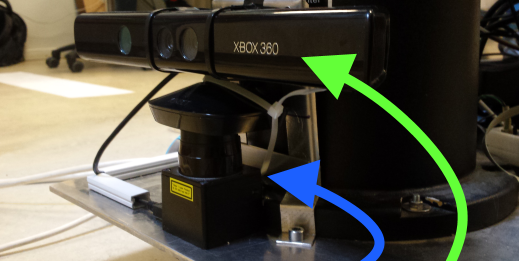
\includegraphics[width=0.8\textwidth]{lidar_and_kinect}
	\caption{Sensor locations for \textcolor{blue}{LIDAR} and \textcolor{green}{Kinect}. }
	\label{fig:kinect_and_lidar}
\end{figure}

\subsection{Sensor Calibration and Setup}

\begin{figure}[h]
	\centering
	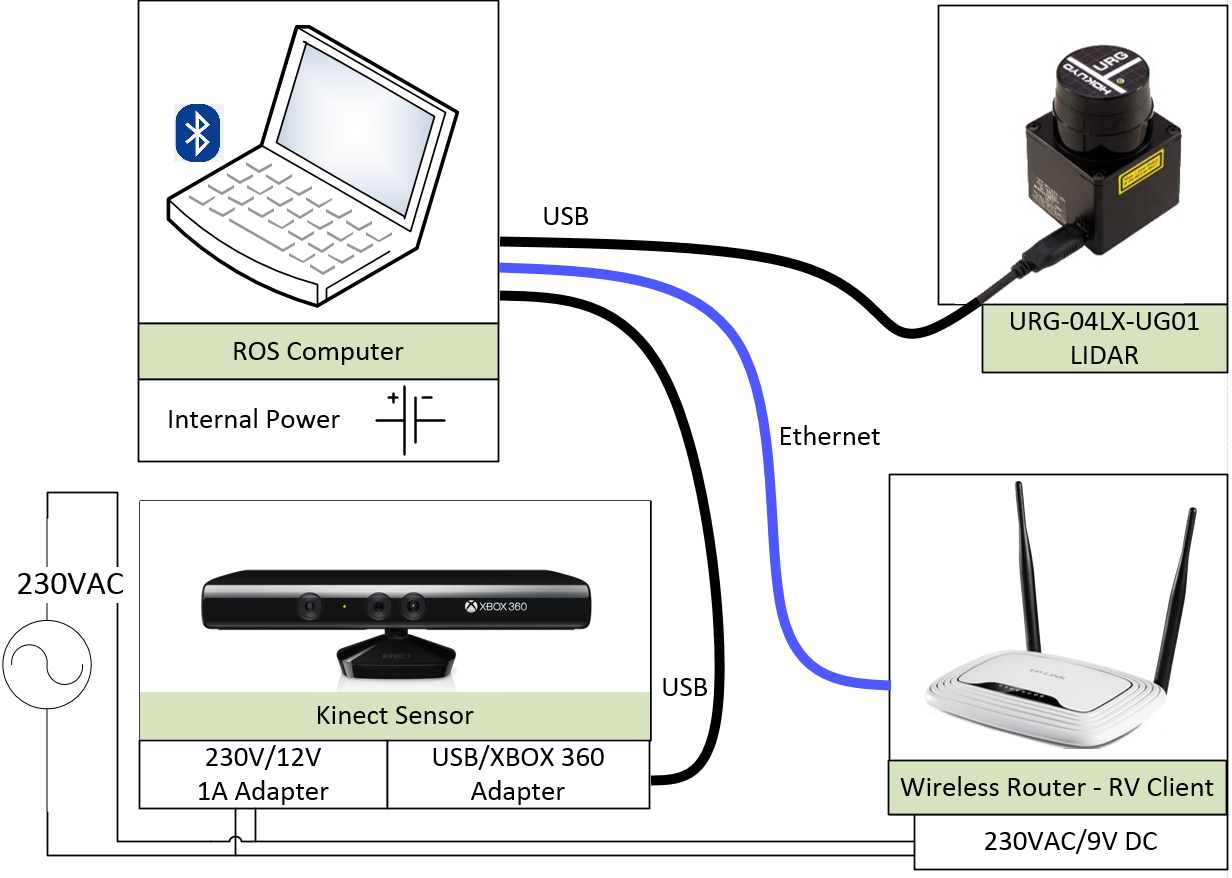
\includegraphics[width=1\textwidth]{sensor_connections}
	\caption{Sensor and power supply connections. }
	\label{fig:sensor_connections}
\end{figure}

Only support for the Kinect and the \ac{LIDAR} sensor was integrated into this system. Odometry from the two wheel encoders was not included because of time constraints on the project. Figure \ref{fig:sensor_connections} illustrates how the sensors and the wireless router is connected to the \ac{ROS} computer and how they are supplied with power.

Calibrating both the Kinect and the \ac{LIDAR} is a straight forward procedure with \ac{ROS}. The Hokuyo \ac{LIDAR} will in fact be calibrated automatically when the node is launched. Calibrating the Kinect is actually not strictly necessary because the lens distortion is very low. However, because there already is a calibration tool available in \ac{ROS}\footnote{ROS calibration guide: \url{http://wiki.ros.org/openni_launch/Tutorials/IntrinsicCalibration}} that is easy to use, there is no good reason to not calibrate. Calibration is highly recommended in the \ac{RTAB-Map} configuration tutorial for \ac{ROS}\cite{rtabmap_setup}. The calibration procedure is as follows:

\begin{enumerate}
	\item Print out a chessboard pattern and tape it to a flat surface. It is beneficial to use a large paper size, for example A3, to make the pattern easier to detect over a larger range of distances.
	\item Calibrate the RGB camera by using the calibration tool. Use the RGB video stream.
	\item Calibrate the IR camera by using the calibration tool. Stream from the IR camera this time. For this procedure, it is recommended to cover the IR projector, because the IR speckle pattern makes it difficult to detect the chessboard (figure \ref{fig:ir_calibration}).
\end{enumerate}

The calibration program needs to know the number of inner corners of the chessboard pattern, and the size of the squares. The chessboard used in this project has $6$ by $9$ inner corners and the size of the squares is $0.0275 m$. Larger pattern squares will make it easier to detect the chessboard pattern over a larger range of distances.

 \begin{figure}[h]
 	\centering
 	\begin{subfigure}[b]{0.47\textwidth}
 		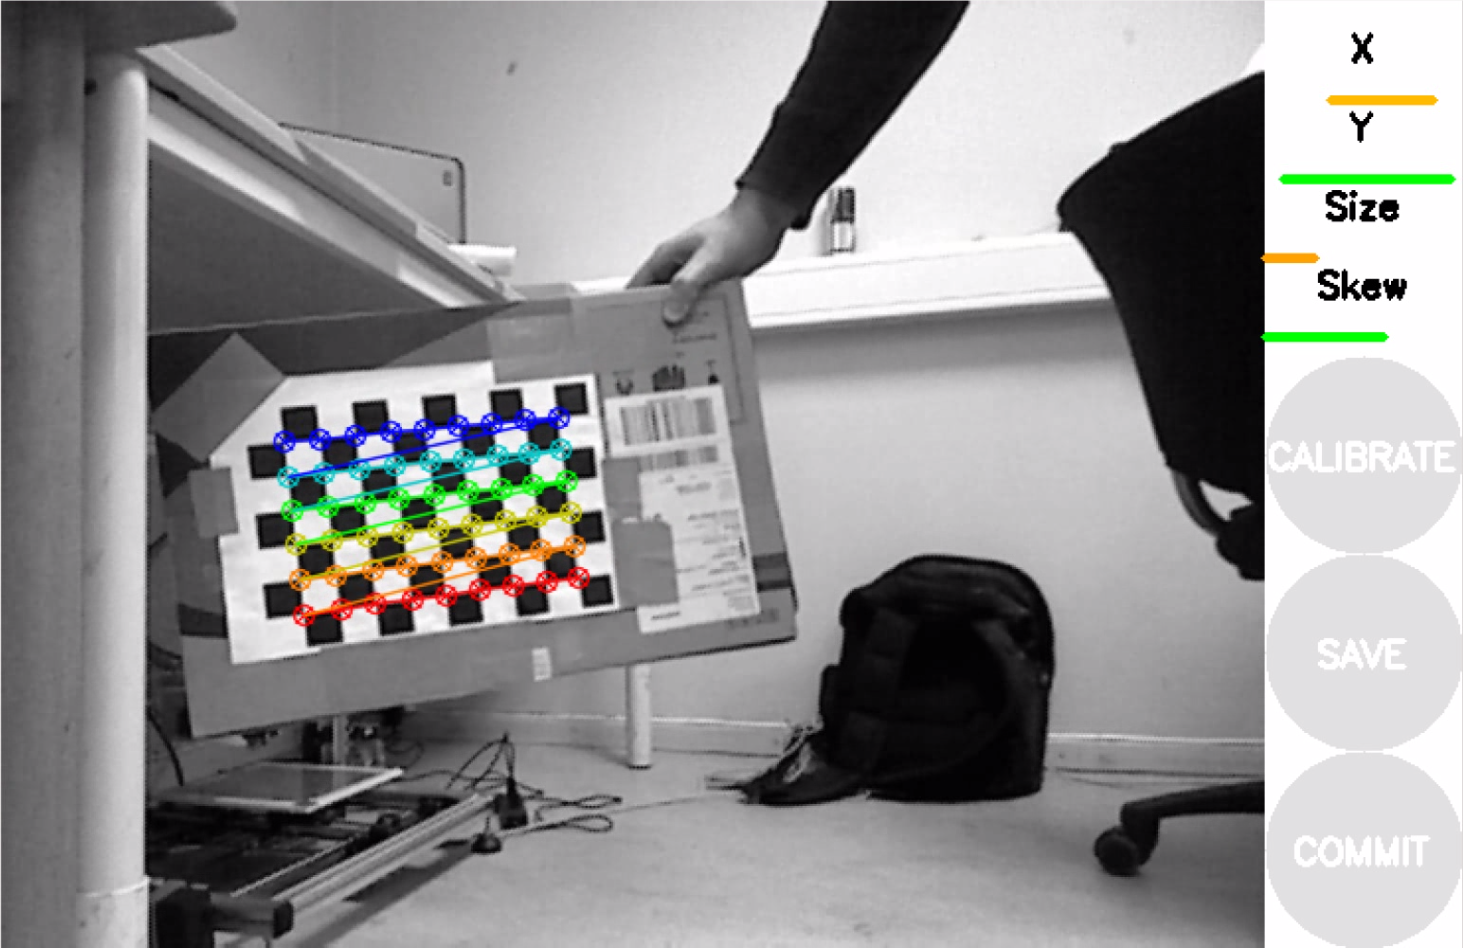
\includegraphics[width=\textwidth]{rgb_calibration}
 		\caption{RGB camera calibration. The camera can be calibrated when a sufficient number of samples have been obtained.}
 		\label{fig:rgb_calibration}
 	\end{subfigure}
 	\begin{subfigure}[b]{0.47\textwidth}
 		
 		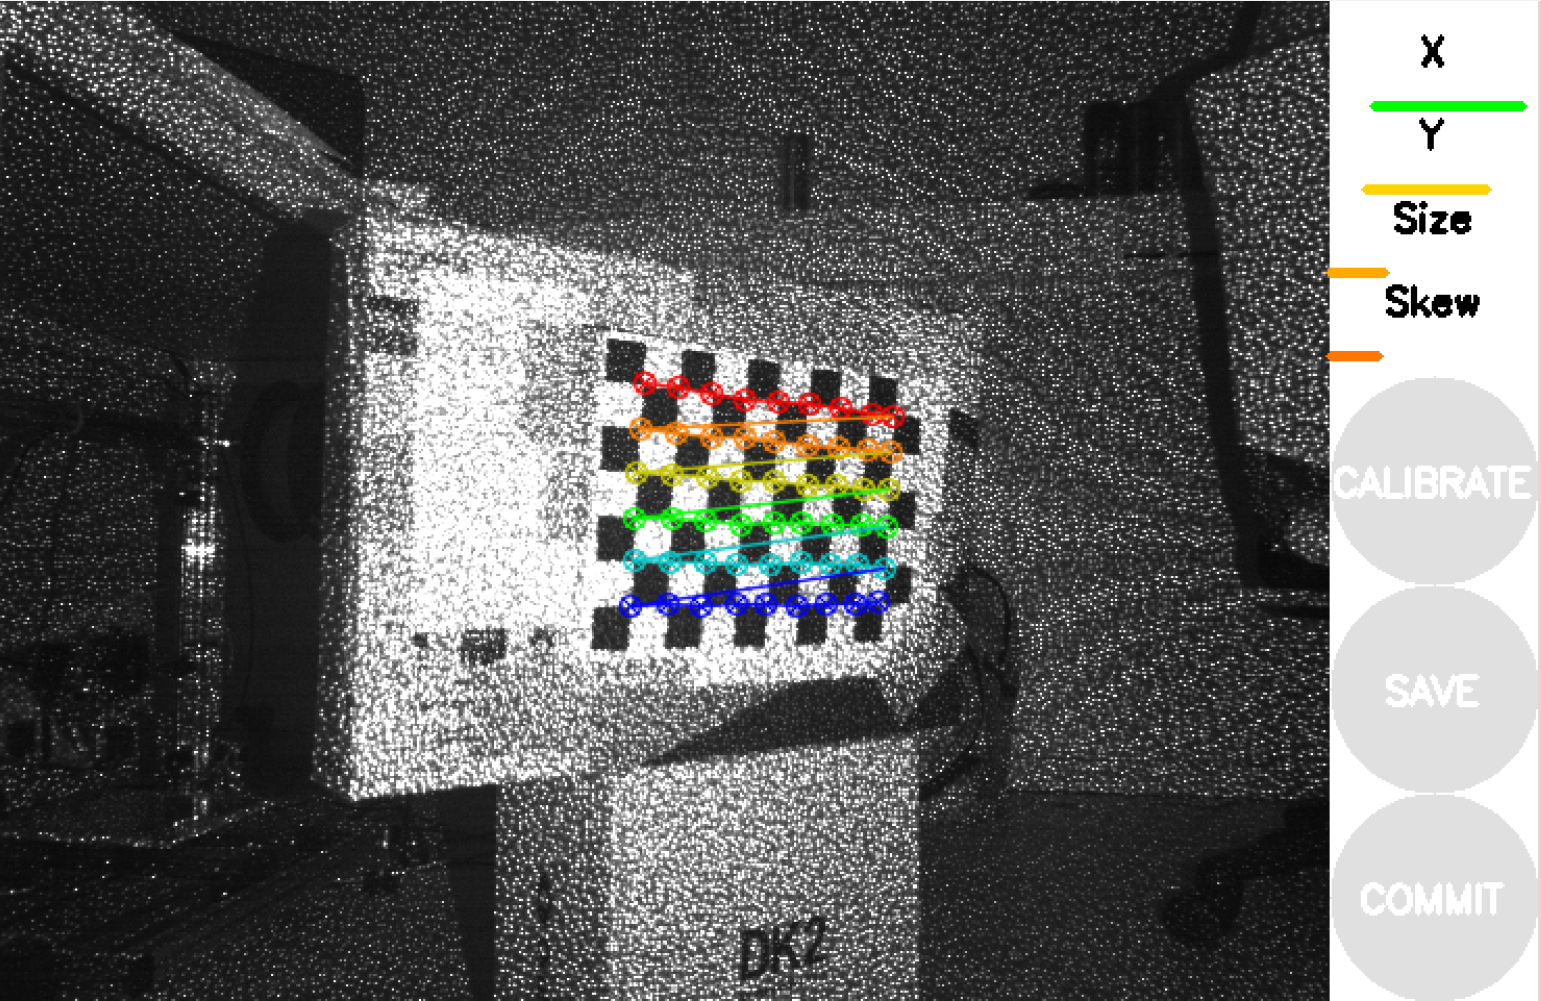
\includegraphics[width=\textwidth]{ir_calibration}
 		\caption{IR camera calibration. The chessboard pattern will be difficult to detect, because the IR projector is not blocked.}
 		\label{fig:ir_calibration}
 	\end{subfigure}
 	\caption{Depth camera calibration.}
 \end{figure}

\subsection{Power Supply and Battery Safety}

This system requires only a subset of the equipment mounted on the robot. A 24V battery used by M. Berg and P. Aspunvik(\cite{berg} and \cite{aspunvik}) is replaced by a $230VAC/24VDC$ converter. Besides the $AC/DC$ converter, the Kinect and wireless router are the only components which require a supply of $230V AC$. A possible power supply setup is shown in figure \ref{fig:power}.

\begin{figure}[h]
	\centering
	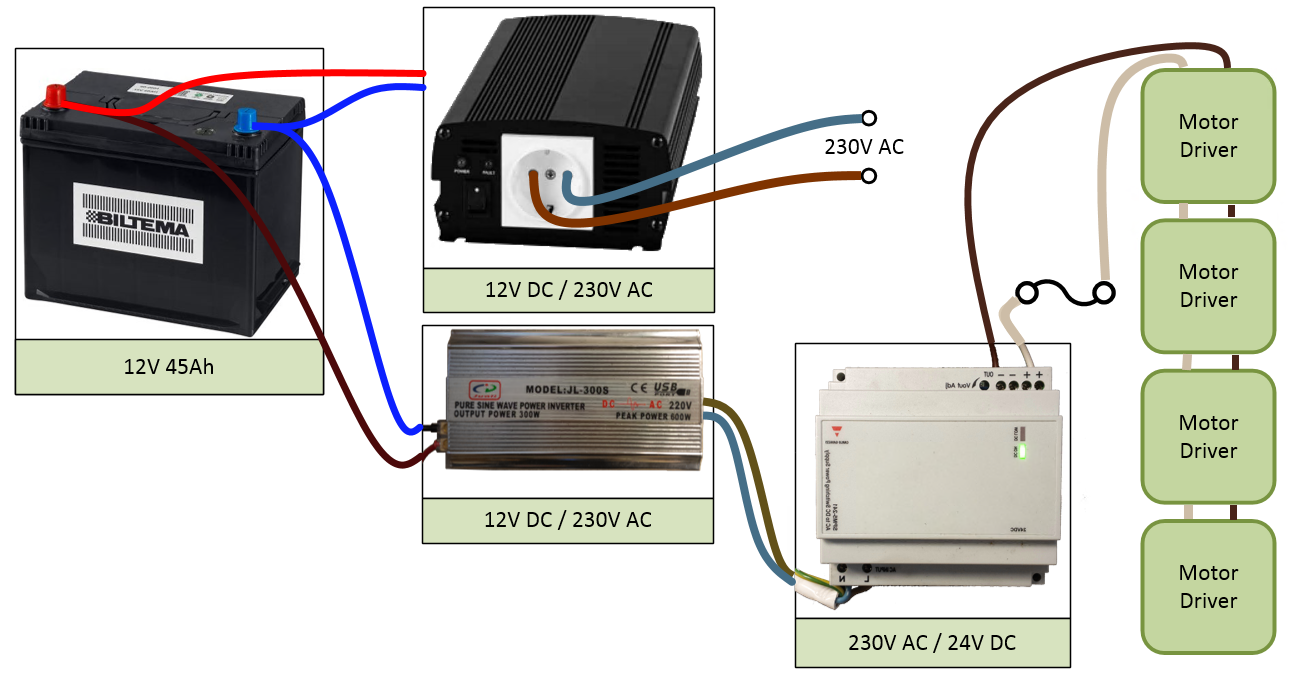
\includegraphics[width=1\textwidth]{power}
	\caption{Example of a feasible power supply setup.}
	\label{fig:power}
\end{figure}

The car battery is now placed in the lower shelf in the rear compartment where it is surrounded by aluminium. This presents an unacceptable risk, because a short circuit is much more likely in this location if the battery poles are uncovered. To reduce the possibility of having a short circuit, an isolating rubber pad was glued to the inner wall and roof next to the battery in the rear compartment. New isolated battery connections provide additional protection. 

\section{ROS Integration Overview}
\label{sec:integration}

The process of integrating \ac{ROS} with the mobile robot platform was influenced by chapter 16 in \cite{rosbook15}, ''Your Own Mobile Robot''. The steps suggested by \cite{rosbook15},  are:

\begin{enumerate}
	
	\item Decide on ROS message interface. Section \ref{sec:control}.
	\item Write interfaces for the motor drivers.
	\item Create a description of the physical structure and properties of the robot in \ac{URDF}. Section \ref{sec:modeling}.
	\item Extend the model to allow simulation in Gazebo.
	\item Publish coordinate transform data via \textit{tf} and visualize it in \texttt{rviz}.
	\item Add sensors, with driver and simulation support.
	\item Apply algorithms for navigation and other functionality. Section \ref{sec:navigation}.
\end{enumerate}



The robot software implementation is placed within a \texttt{catkin} workspace (see section \ref{sec:catkin}) that contains all the project specific files that are necessary to build and run the robot system. The overarching file system is shown in figure \ref{fig:file_system}. Note that there are several references to the \ac{TLA} ''mar'', which is short for \ac{MAR}.

\begin{figure}[h]
	\centering
	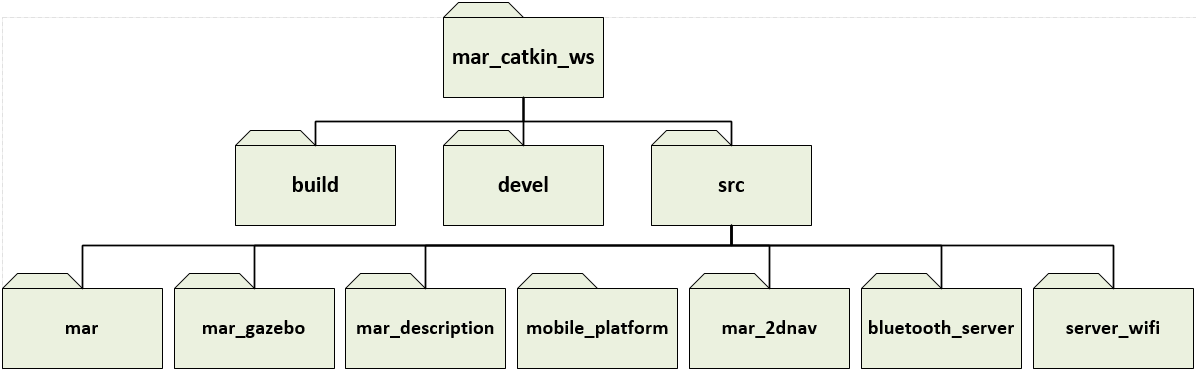
\includegraphics[width=1\textwidth]{file_system}
	\caption{Overarching file system. The \ac{ROS} packages are located within \texttt{src}.}
	\label{fig:file_system}
\end{figure}

Each package will be introduced in the following sections. The purpose of presenting the file systems is to clarify which parts of the system that was implemented by this author. A short description of each package is given in table \ref{tab:list_packages}, and their place in the workspace hierarchy is shown in figure \ref{fig:file_system}.

\begin{table}
	\centering
	\begin{tabular}{ r p{8.5cm} }
		\hline
		\multicolumn{2}{c}{Packages within \texttt{mar\_catkin\_workspace}}\\
		\hline
		\texttt{mar} & Launch files for the real robot hardware and for \ac{RTAB-Map}.\\
		\texttt{mar\_gazebo} & Launch files for the simulated robot and for \ac{RTAB-Map}.\\
		\texttt{mar\_description} & \ac{URDF} files for both the simulated and the real robot.\\
		\texttt{mobile\_platform} & Programs for handling and processing velocity commands. One such node serves as an interface to the motor control card.\\
		\texttt{mar\_2dnav} & Configuration and launch files for both the real and simulated robot.\\
		\texttt{bluetooth\_server} & A node that serves as a Bluetooth server based on the Qt5 API.\\
		\texttt{server\_wifi} & Contains the node responsible for communicating with the \ac{OCS}.\\
		\hline
	\end{tabular}
	\caption{List of custom made packages.}\label{tab:list_packages}
\end{table}


\section{Modeling}
\label{sec:modeling}
A robot model will serve two purposes in this implementation. First of all, the system needs a definition of how the sensor inputs are placed with respect to the \texttt{base\_link}. The origin of \texttt{base\_link} is associated  with a coordinate frame. This frame, and any other frame in \ac{ROS}, is right handed, i.e. the positive $x$ direction is \textit{forwards}, positive $y$ points \textit{left}, and positive $z$ is \textit{up}. The robot pose will be based on the transformation between the world and the \texttt{base\_link} frame. 

The second purpose of the model is simulation. Being able to simulate the robot system has been invaluable throughout this project. The robot model is represented in an XML-based modeling language called \ac{URDF} (Unified Robot Description Format). There are two \textit{.urdf} files within the package \texttt{mar\_description}; one for the simulator and one for the real robot hardware. The following sections presents how these models were defined.


\subsection{Physical Dimensions}

Step one in building the model was to define its geometrical shape. The current model shape consists of several links. Each link is defined as a shape and a size. The links are connected together by joints that define the coordinate transformation between the links. All links were modeled as either cuboids or cylinders, in order to simplify and speed up the modeling process. All joints are static except for the wheels which are continuous joints. For simplicity, the robot arm is modeled by a dummy link with the shape of a cylinder.

\begin{figure}[h]
	\centering
	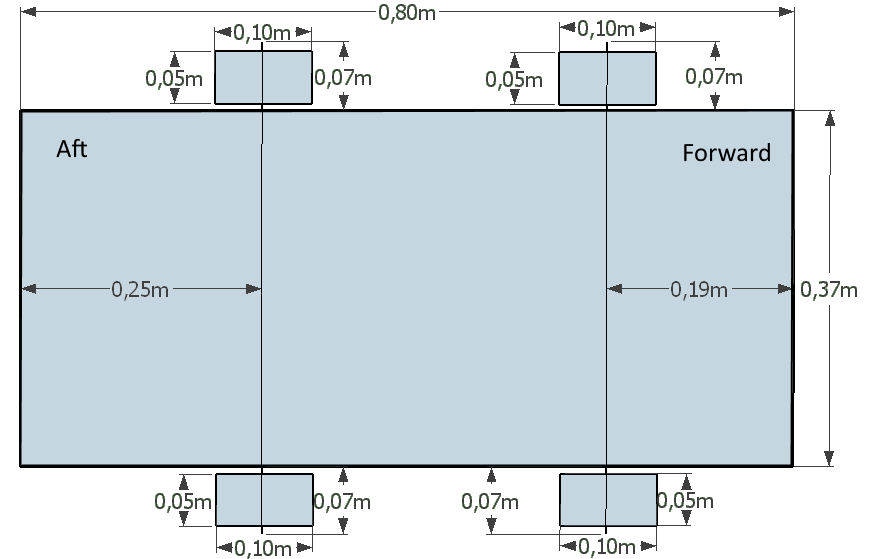
\includegraphics[width=0.85\textwidth]{robotFootprint2}
	\caption{The robot footprint. Dimensions are used for the navigation planners and for modeling. }
	\label{fig:robotFootprint}
\end{figure}

After defining the model shape, it is time to add some additional physical attributes to each link. Each link requires an inertia tensor in order to simulate the model. It is also useful to define a collision volume for each link. In this model, the collision volume is equal to the geometric shape of the link without exceptions. Inertia tensors for each shape is based on equations \ref{eq:cylinder} or \ref{eq:cuboid}.

The inertia tensor:

\begin{equation}
    	I = \begin{bmatrix}
    	I_{xx} & I_{xy} & I_{xz} \\[0.3em]
    	I_{yx} & I_{yy} & I_{yz} \\[0.3em]
    	I_{zx} & I_{zy} & I_{zz}
    	\end{bmatrix}
\end{equation}

Inertia tensor for a solid, uniform cylinder where the radius $r$ is measured in parallel to the $x - y$ plane, and $h$ is parallel to the $z$ axis:
\begin{equation}
I_{cylinder} = \frac{1}{12}m \begin{bmatrix}
	(3 r^2 + h^2) & 0 & 0 \\[0.3em]
	0 & (3 r^2 + h^2) & 0 \\[0.3em]
	0 & 0 & 6r^2
	\end{bmatrix}
	\label{eq:cylinder}
\end{equation}

Inertia tensor for a solid, uniform cuboid. The subscript of $l$ indicates which axis $l$ is measured along:
\begin{equation}
I_{cuboid} = \frac{1}{12}m \begin{bmatrix}
	(l_y^2 + l_z^2) & 0 & 0 \\[0.3em]
	0 & (l_x^2 + l_z^2) & 0 \\[0.3em]
	0 & 0 & (l_x^2 + l_y^2)
\end{bmatrix}
\label{eq:cuboid}
\end{equation}

The mass of each link is guesstimated. Consider the \texttt{base\_link} as an example. The base link was measured to be $5 \; mm$ thick, $37 \; cm$ wide and $80 \; cm$ long. Assuming that the density of aluminium\footnote{https://en.wikipedia.org/wiki/Aluminium} is $2.7 g/cm^3$, the mass of this link was calculated to be $\approx 4 kg$. The base link was defined as follows:

\lstset{language=XML}
\begin{lstlisting}
<link name="base_link">
  <visual>
    <geometry>
      <box size="0.8 0.37 0.005"/>
    </geometry>
    <material name="silver"/>
  </visual>
	  
  <collision>
    <geometry>
      <box size="0.8 0.37 0.005"/>
    </geometry>
  </collision>
	  
  <inertial>
    <mass value="4" />
    <origin xyz="0 0 0" />
    <inertia ixx="0.04564" ixy="0.0" ixz="0.0"
      iyy="0.21334" iyz="0.0" 
      izz="0.25879" />
  </inertial>
</link>
\end{lstlisting}

\subsection{Connecting the Links}

Robot links are connected by joints. A joint defines a translation and rotation from the coordinate frame of a parent link to that of a child link. Each joint has two attributes: \textit{name}, for example ''base\_link\_to\_left\_wheel'' and type, for example ''prismatic'' or ''continuous''. All joints in the mobile robot are static, except for the wheel joints which are continuous. Correct joint transformations is very important when placing the sensors (figure \ref{fig:sensor_frames}). A discrepancy between the real sensor-to-base transform and the modeled transform will cause misaligned sensor input.

 \begin{figure}[h]
 	\centering
 	\begin{subfigure}[b]{0.402\textwidth}
 		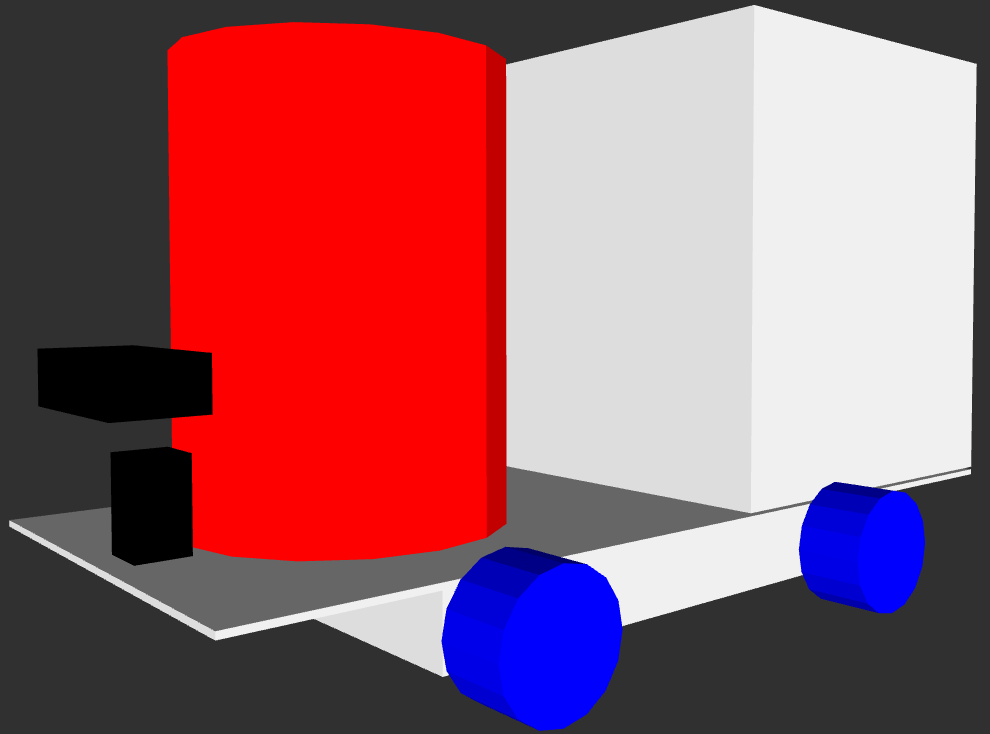
\includegraphics[width=\textwidth]{urdf_model}
 		\caption{Complete \ac{URDF} model when viewed in \texttt{rviz}.}
 		\label{fig:urdf_model}
 	\end{subfigure}
 	\begin{subfigure}[b]{0.51\textwidth}
 		
 		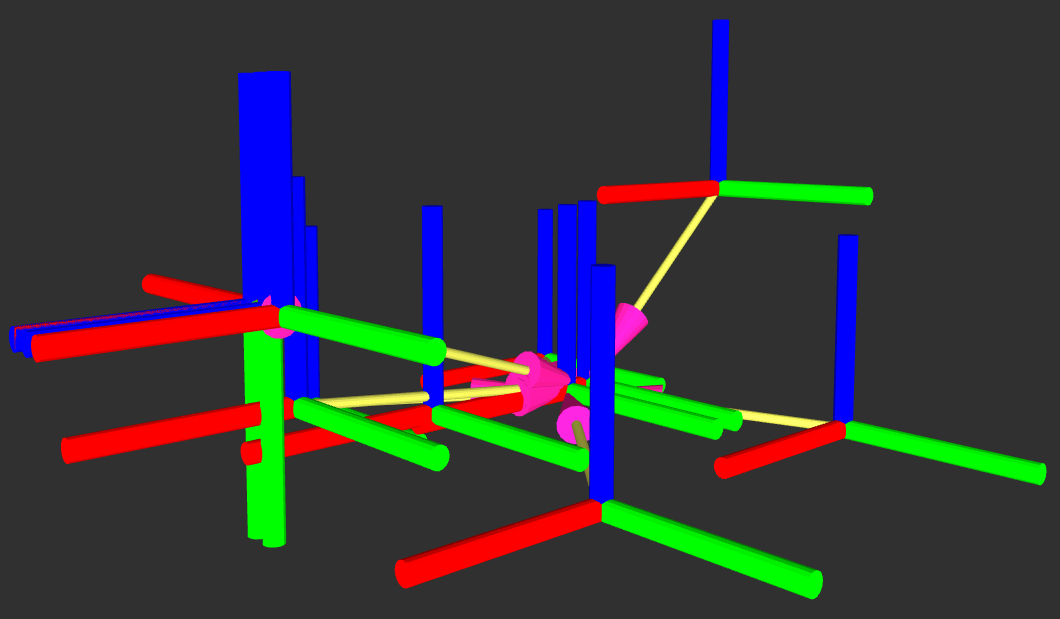
\includegraphics[width=\textwidth]{urdf_tf2}
 		\caption{\ac{URDF} model in \texttt{rviz} with all link frames and transformations.}
 		\label{fig:urdf_tf}
 	\end{subfigure}
 	\caption{\ac{URDF} model.}
 \end{figure}

\begin{figure}[h]
	\centering
	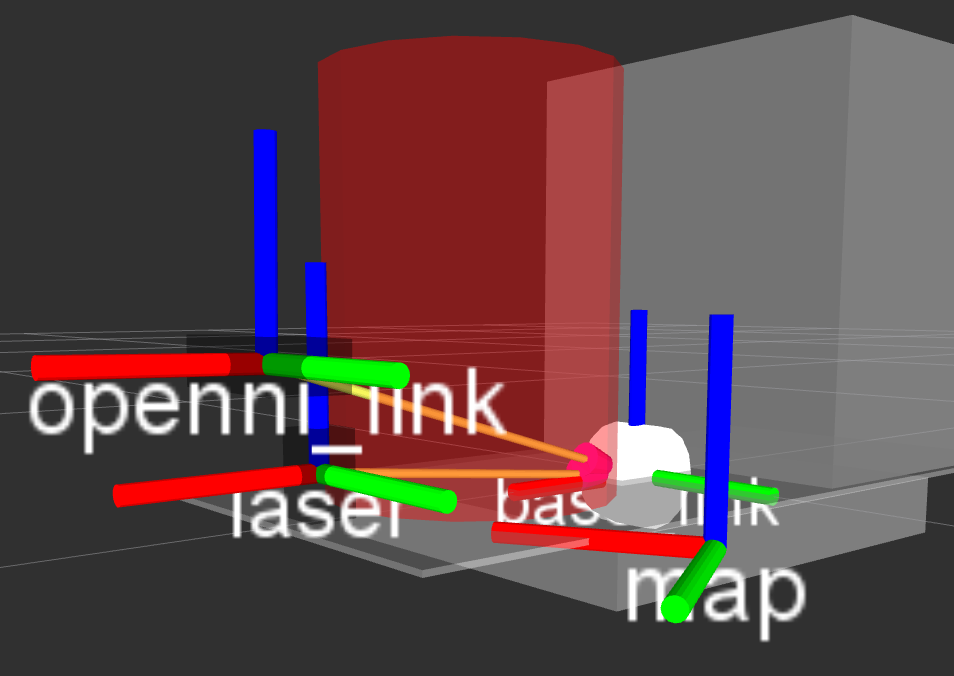
\includegraphics[width=0.5\textwidth]{sensor_frames}
	\caption{Robot model with frames for laser, Kinect, robot base and map. }
	\label{fig:sensor_frames}
\end{figure}

\begin{figure}[h]
	\centering
	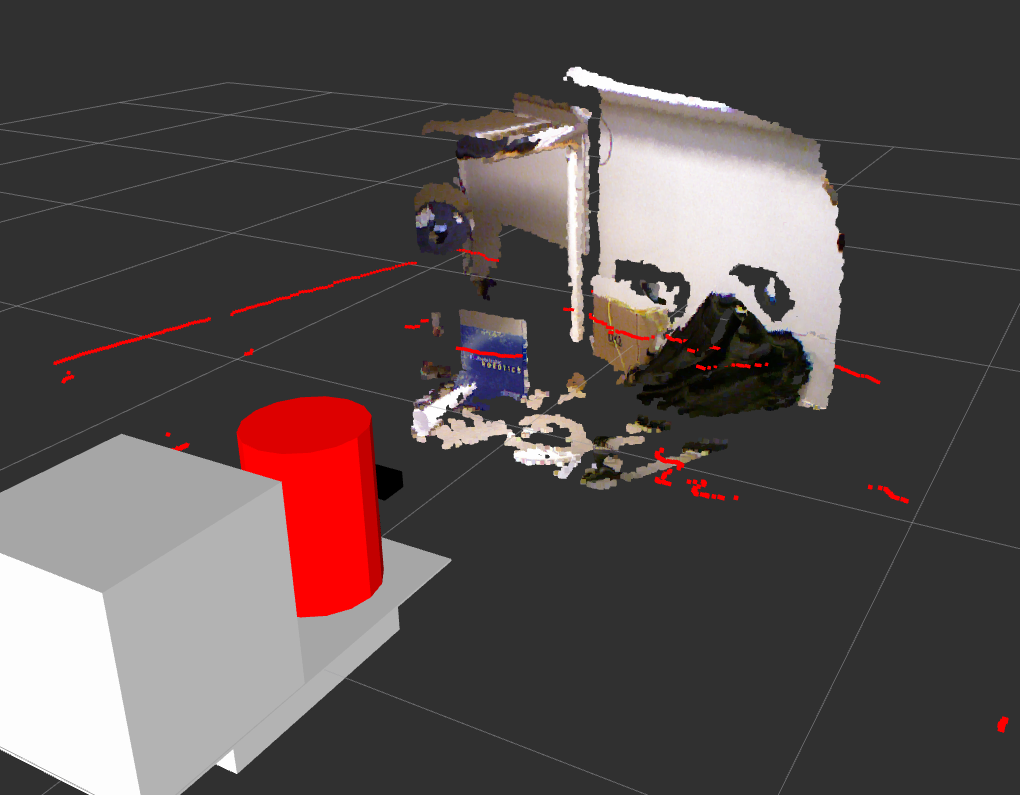
\includegraphics[width=0.5\textwidth]{sensors_in_frame}
	\caption{Sensor input placed with correct transformations from \texttt{base\_link}. }
	\label{fig:sensors_in_frame}
\end{figure}


\section{Simulations}
\label{sec:simulations}
Robot simulation was done in Gazebo; a simulation tool with good interfaces to \ac{ROS}. The same \ac{ROS} graph was used for both the simulated and real version of the robot, except from the sensors and actuators, and some minor parameter changes. 

\begin{figure}[h]
	\centering
	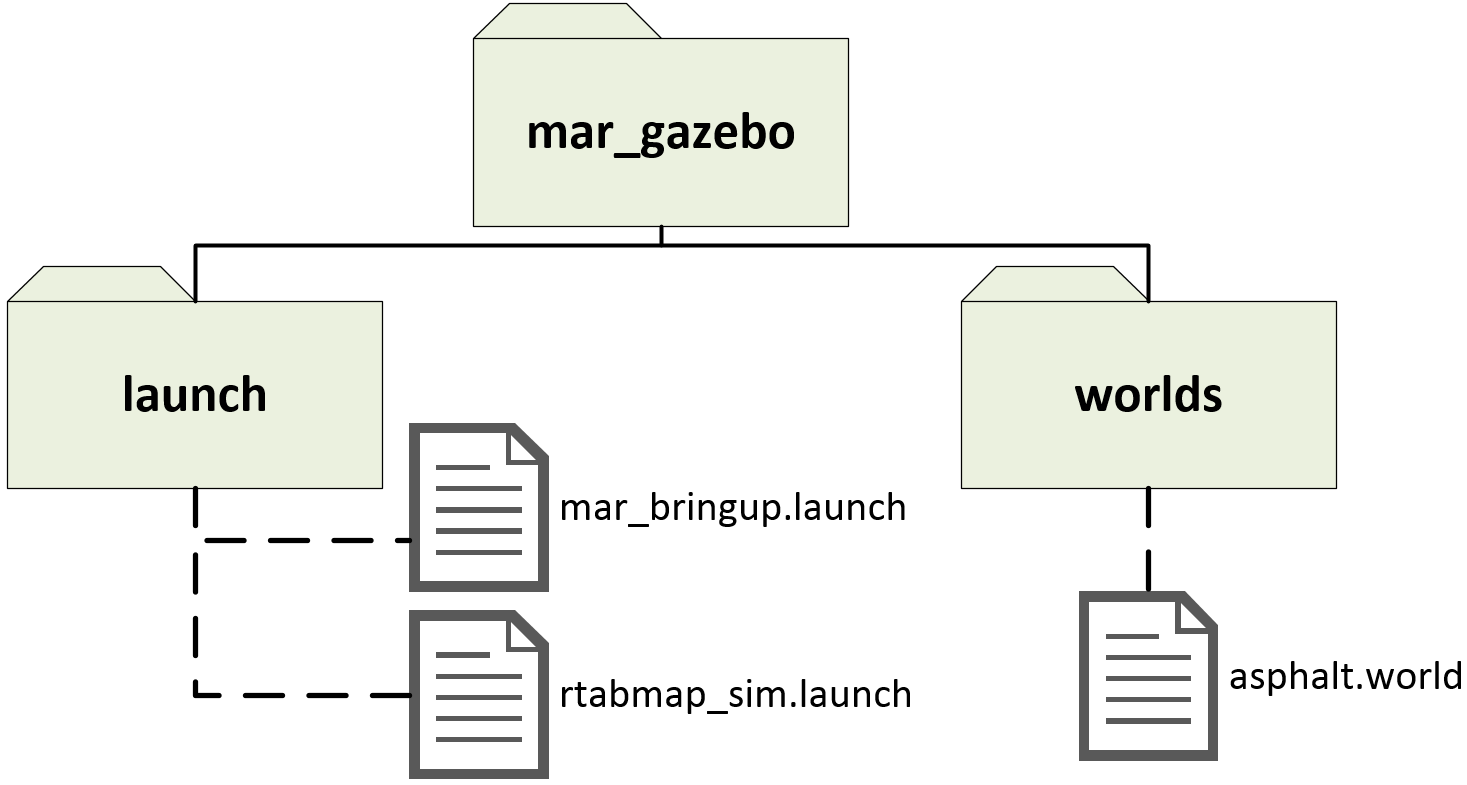
\includegraphics[width=0.7\textwidth]{mar_gazebo_folders}
	\caption{Folders and files specific for the simulator.}
	\label{fig:mar_2dnav}
\end{figure}

To properly simulate the robot, Gazebo needs a way to simulate the differential drive and the sensors in addition to the physical description of the robot. An expanded \ac{URDF} description of the robot, \texttt{mar\_model\_sim.urdf}, intended for Gazebo was placed within the \texttt{mar\_description} package (figure \ref{fig:file_system}). 

\subsection{Robot Description Plugins}

The \ac{URDF} model in \texttt{mar\_model\_sim.urdf} was expanded with plugins that simulate the motor control card, the \ac{LIDAR} and the Kinect. The plugins are provided by Gazebo and are intended for use in \ac{ROS}. 

The motor controller is simulated by the \texttt{skid\_steer\_drive\_controller} plugin. This plugin was preferred over the \texttt{differential\_drive\_controller} because it supports four wheel joints instead of two, and because the skid steering controller was considered to be good enough. 

Attributes for gazebo's sensor plugins are based on the technical specifications\cite{hokuyo_spec} for the real sensors. 

\section{ROS Nodes for Motion Control}
\label{sec:control}
All nodes for motion control are located within the package \texttt{mobile\_base}. This package is organized as shown in figure \ref{fig:mobile_platform_files}.

\begin{figure}[h]
	\centering
	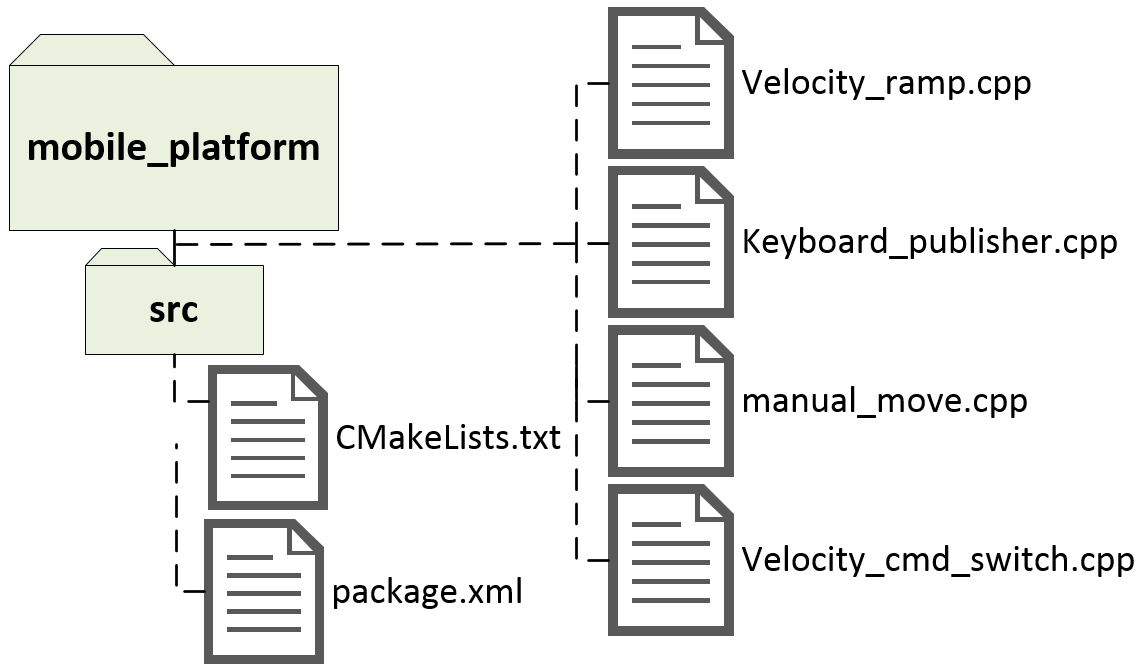
\includegraphics[width=0.65\textwidth]{mobile_platform_files}
	\caption{Files within the package \texttt{mobile\_platform}.}
	\label{fig:mobile_platform_files}
\end{figure}

\subsection{Velocity Command Flow}

There are four sources that can generate velocity commands for the robot. Common for all of these is that they use the message format \texttt{geometry\_msgs/Twist}. The names for each of the four velocity messages are as follows:

\begin{description}
	\item[/cmd\_vel\_loc] Local keyboard input.
	\item[/cmd\_vel\_wifi] Wireless teleoperation from the \ac{OCS}.
	\item[/cmd\_vel\_bt] Wireless teleoperation from a hand-held Bluetooth device.
	\item[/cmd\_vel] Commands from the navigation stack in \ac{ROS}. \texttt{/cmd\_vel} is the default \: \: velocity command topic for the navigation stack.
\end{description}

The third topic \texttt{/switch\_setting} is a command used to select the velocity command to be passed all the way to the motor control card, or Gazebo in the case of a simulated session. The message flow between source and sink is illustrated as a \ac{ROS} graph in figure \ref{fig:move_base_nodes}.

\begin{figure}[h]
	\centering
	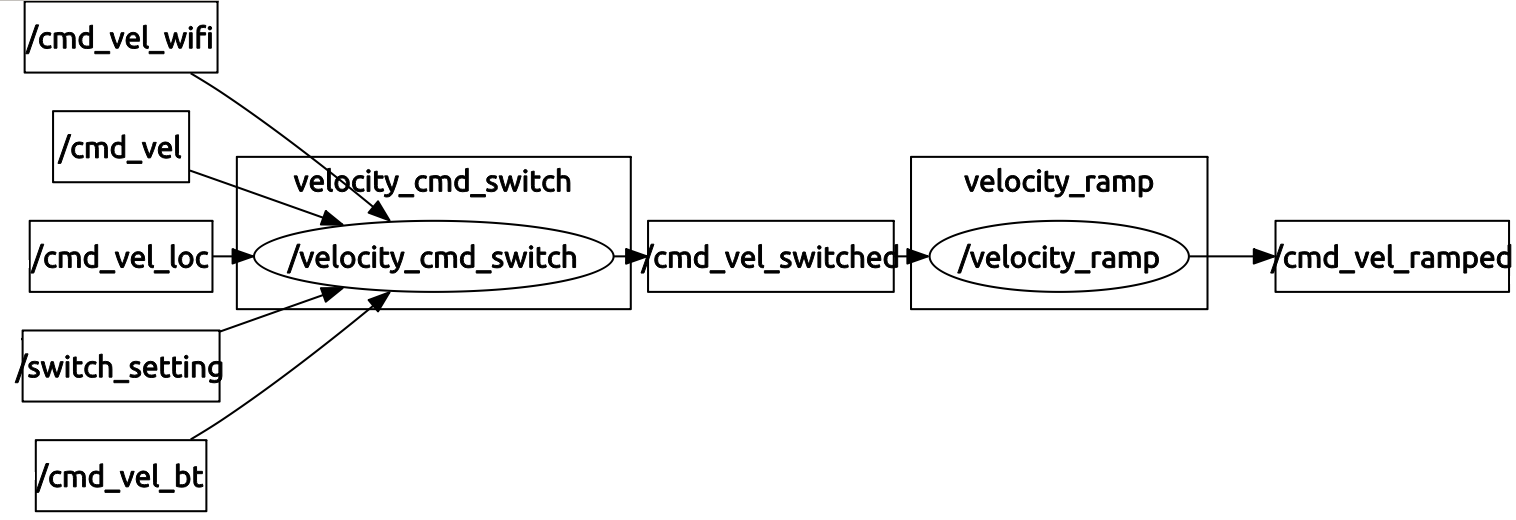
\includegraphics[width=1\textwidth]{velocity_command}
	\caption{Nodes and topics for motion control. (see figure \ref{fig:minimum_graph} for an explanation of this figure).}
	\label{fig:move_base_nodes}
\end{figure}

Rapid changes in the velocity command may cause excessive wear and tear on the equipment. The node \texttt{velocity\_ramp} has been added to ensure that the velocity command values will change smoothly. Implementation of this node is heavily based on example code from \cite{rosbook15}. The example code was translated from Python to C++, and adapted to fit into this particular system. Figure \ref{fig:velocity_ramp} shows an example of how \texttt{velocity\_ramp} works.

\begin{figure}[h]
	\centering
	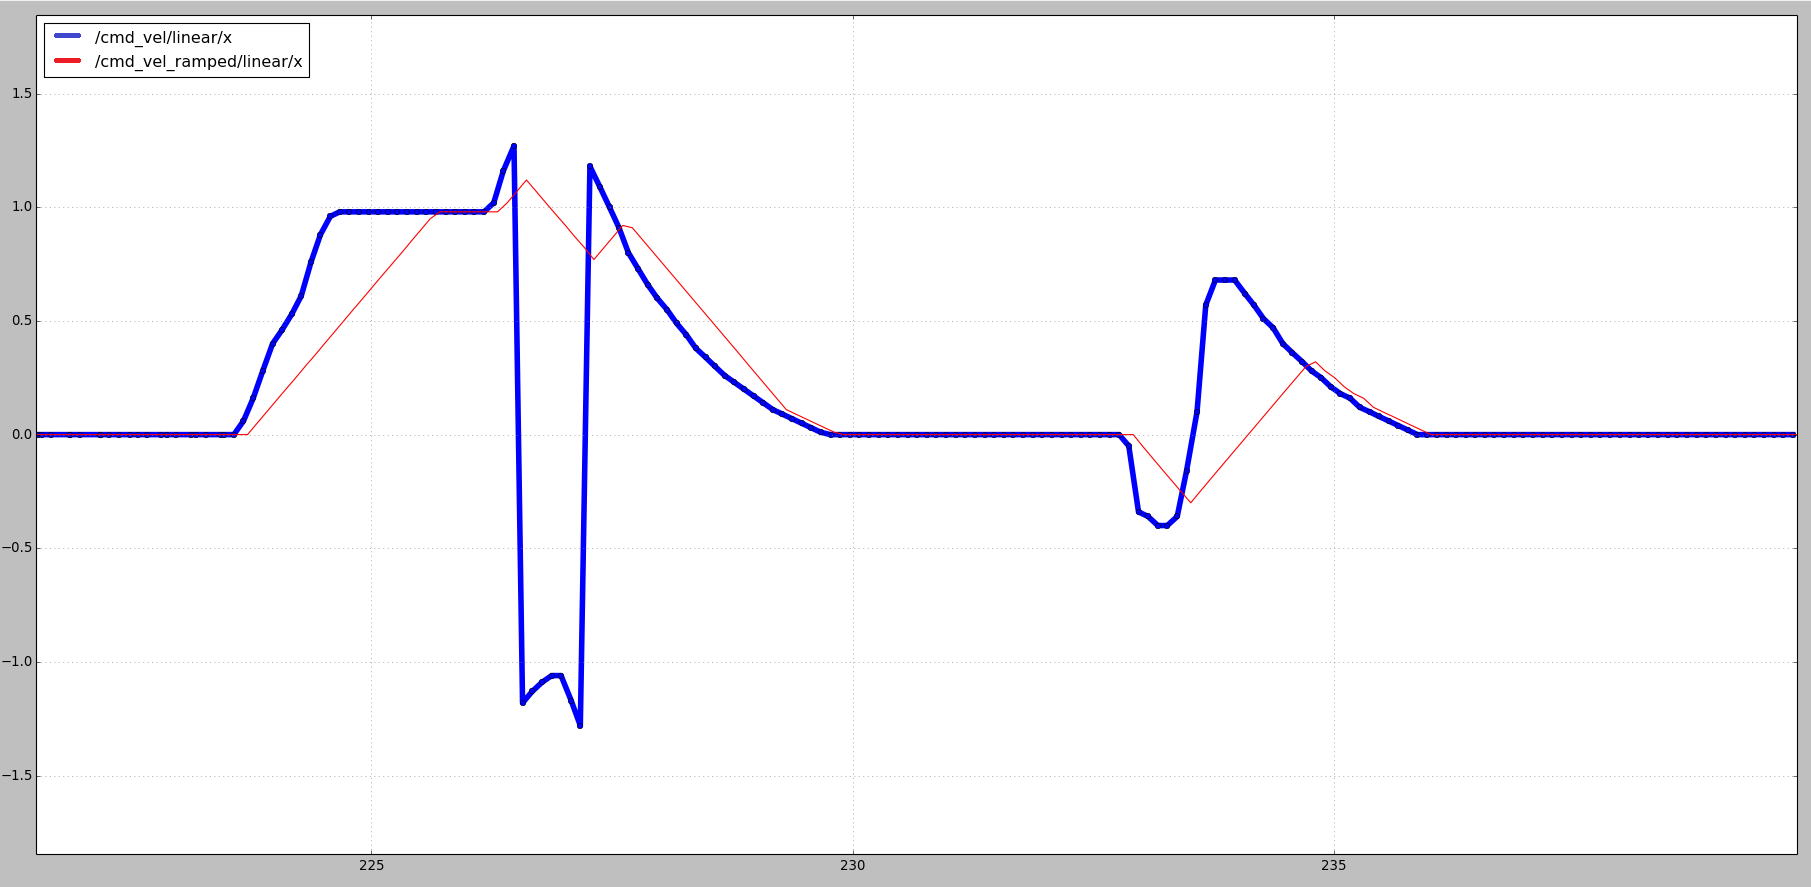
\includegraphics[width=1\textwidth]{velocity_ramp_cropped}
	\caption{The node \texttt{velocity\_ramp} limits the rate of change of the velocity command sent to the motor control card. The blue line represents commands entering \texttt{velocity\_ramp}, while the red line shows the acceleration constrained output command.}
	\label{fig:velocity_ramp}
\end{figure}


\subsection{Motor Control Card Firmware on XMEGA A3BU}

XMEGA A3BU is an evaluation board developed by Atmel. The The implementation presented here is an adaptation of Petter Aspunviks implementation \cite{aspunvik}. The following paragraphs presents the most significant firmware changes that were made.

The firmware will now receive angular and linear velocity commands based on the \texttt{geometry\_msgs/Twist} message format in \ac{ROS}, and translate these into the command format used by each motor. Speed settings for each motor is based on \ac{PWM}. 

There were two requirements for this implementation: 
\begin{enumerate}
\item When velocity commands from the operating system are either absent or incomplete, the robot shall stop.
\item The program shall translate linear and angular velocity commands into wheel commands.
\end{enumerate}

\begin{figure}[h]
	\centering
	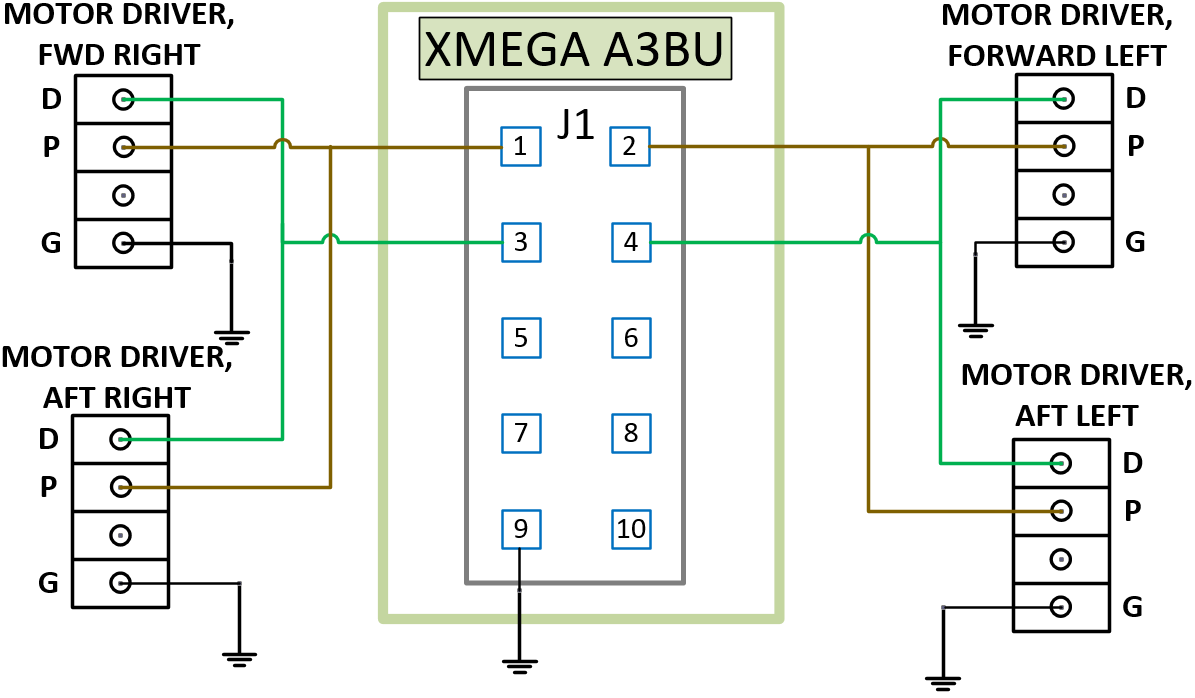
\includegraphics[width=0.9\textwidth]{conn_diag_motors}
	\caption{Connections between each wheel motor driver and the motor control card, XMEGA A3BU. The connections are unchanged from \cite{aspunvik}, except for some improved connection for better short circuit prevention.}
	\label{fig:conn_diag_motors}
\end{figure}

The connections in figure \ref{fig:conn_diag_motors} are the same as in \cite{aspunvik}, except for the installation of more secure connections under the robot. The old connections were insecure, and the risk of short circuits was substantial.

\subsubsection{ROS-Motor Driver Communication}

Communications between the motor control card and \ac{ROS} is done via a USB serial port. The node \texttt{motor\_driver\_interface} within the package \texttt{mobile\_platform} is responsible for transmitting velocity commands via the comport. The node is hard-coded to communicate via \texttt{/dev/ttyACM1}.  The velocity update transmission cycle is shown as a sequence diagram in figure \ref{fig:motor_cmd_sequence}. The transmission cycle is initiated each time \texttt{motor\_driver\_interface} receives a velocity message on the topic \texttt{/cmd\_vel\_ramped}.

\begin{figure}[h]
	\centering
	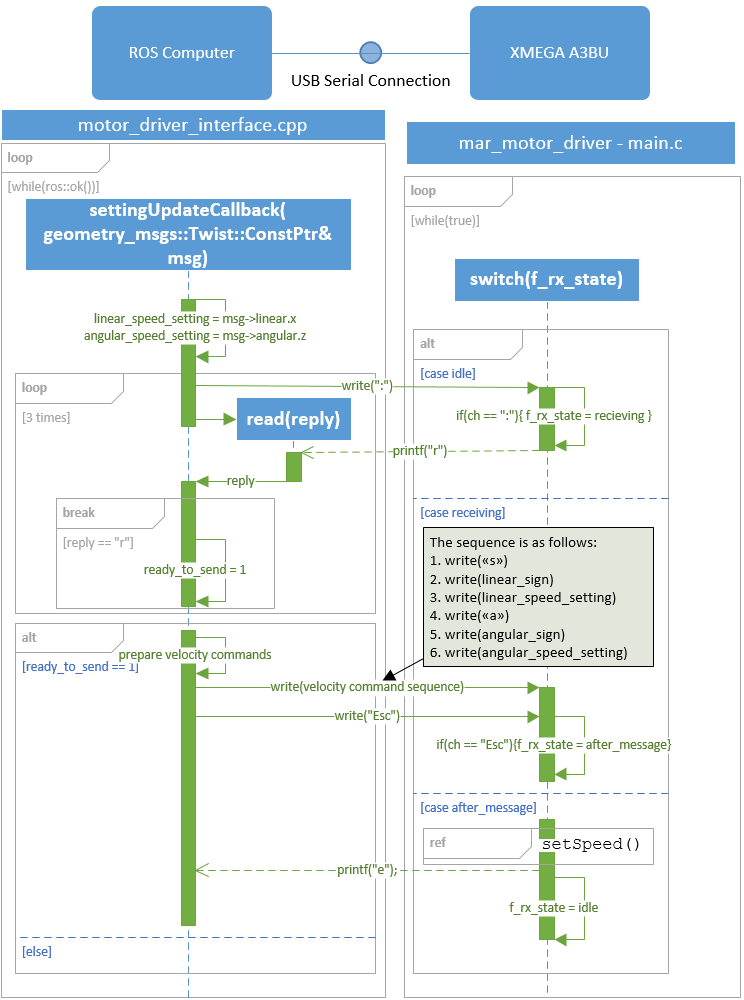
\includegraphics[width=1\textwidth]{motor_cmd_sequence}
	\caption{Velocity command transmission sequence from the \texttt{motor\_driver\_interface} in the ROS computer to the motor control card (XMEGA A3BU).}
	\label{fig:motor_cmd_sequence}
\end{figure}

\subsubsection{From Velocity Commands to Wheel Commands}
\label{sec:velocity2wheels}
Within \ac{ROS}, velocity commands are passed around between nodes in the form of the message \texttt{geometry\_msgs/Twist}. This message type can be viewed as a \textit{struct} with the following contents:

\begin{verbatim}
	Vector3  linear
	Vector3  angular
\end{verbatim}

where each vector contains float values for the directions $x$, $y$ and $z$ with respect to the robot's base frame. Because of the motion constraints of this robot, only \texttt{linear.x} and \texttt{angular.z} are of relevance, and the data which is passed to the motor control card (XMEGA A3BU) is therefore limited to these two values. The motor control card must now translate the linear and angular velocities into wheel speeds. Next, these speeds must be related to a duty cycle for the \ac{PWM} signal which controls each of the four motors.

To perform the translation, it is assumed that the mobile base can be described as a vehicle with differential drive steering. Wheel commands will only distinguish between left or right - not front or aft. Equations of motion which relates angular and linear velocity to wheel velocities can be found in\cite{cook2011mobile}, and are shown below:

\begin{subequations}\label{eq:subeqns}
  	\begin{align}
	  	\omega &= \dot{\psi} \\
	   	v_{left} &= \omega (R - W/2)\\
	   	v_{right} &= \omega (R + W/2) \label{eq:subeq2}
   	\end{align}
\end{subequations}

$W$ is the spacing between the wheels as shown in figure \ref{fig:robot_kinematics}. In \cite{cook2011mobile}, the parameter $R$ represents the instantaneous radius of curvature of the robot trajectory. This mouthful will be substituted by the linear velocity $v$ in the following equations, because $v = R\omega$ (similar to the linear speed of a wheel). This yields two equations for the wheel speeds, $v_{left}$ and $v_{right}$, based on angular and linear velocity, $w$ and $v$.

 \begin{subequations}%\label{eq:subeqns}
 	\begin{align}
 	v &= R\omega \\
 	v_{left} &=  \frac{2v - \omega W}{2}\\
 	v_{right} &= \frac{2v + \omega W}{2} %\label{eq:subeq2}
 	\end{align}
 \end{subequations}

 \begin{figure}[H]
 	\centering
 	\begin{subfigure}[b]{0.58\textwidth}
 		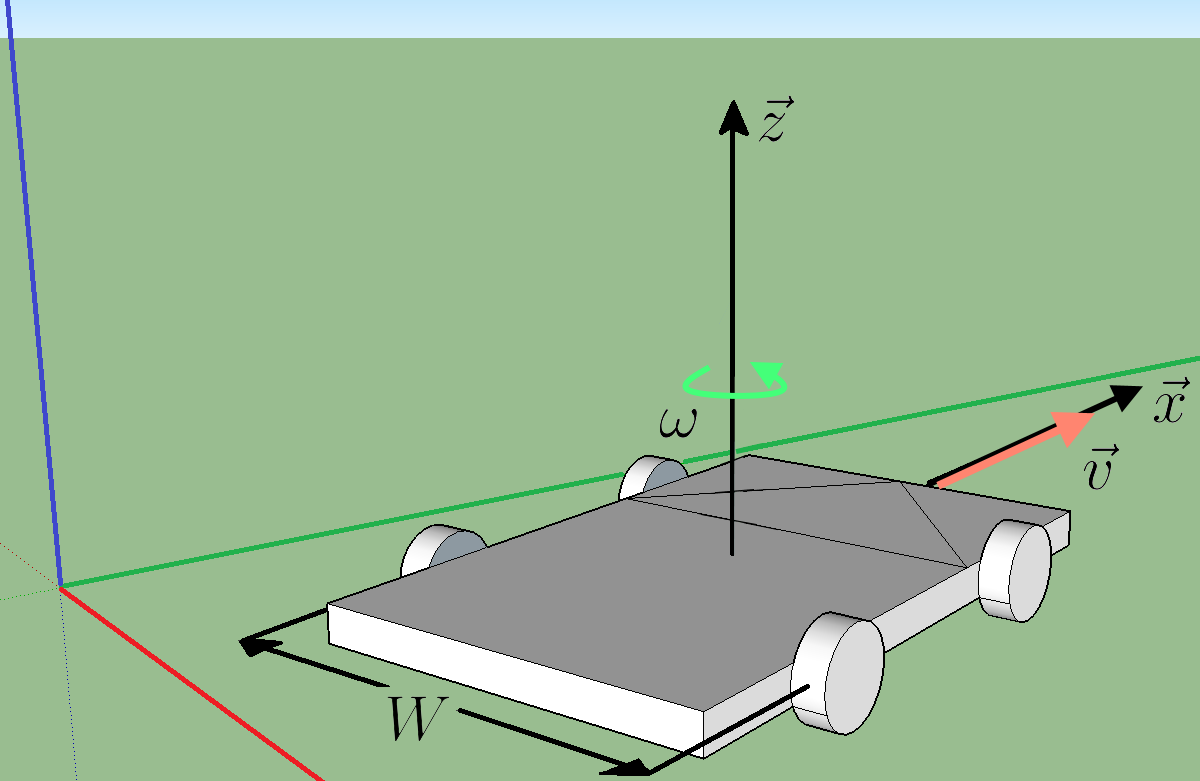
\includegraphics[width=\textwidth]{robot_kinematics2}
 		\caption{Differential drive parameters.}
 		\label{fig:robot_kinematics}
 	\end{subfigure}
 	\begin{subfigure}[b]{0.38\textwidth}
 		
 		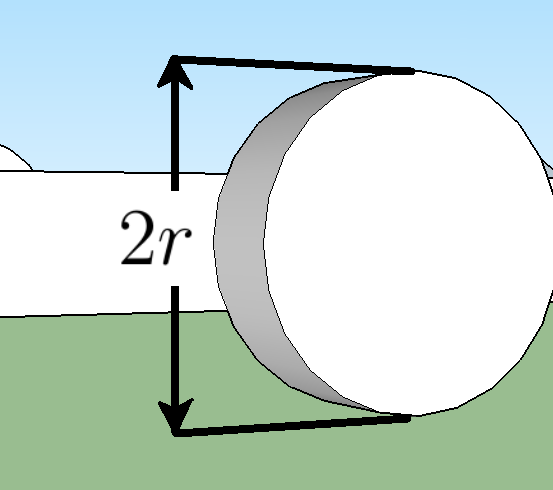
\includegraphics[width=\textwidth]{wheel_diameter}
 		\caption{Wheel diameter.}
 		\label{fig:wheel_diameter}
 	\end{subfigure}
 	\caption{\label{fig:wheel_diameter}Parameters for differential drive kinematics. Note that the frame vectors $\vec{z}$ and $\vec{x}$ refer to the base frame of the robot in this case, and not the world frame.}
 \end{figure}

A wheel command update cycle will begin, on the motor control card, when a new velocity setting is received from \ac{ROS}. After receiving the ''end-of-message'' token, ''\texttt{Esc}'', the receiver state machine will switch to the \texttt{after\_message} state (see figure \ref{fig:motor_cmd_sequence}). Three things will happen within the \texttt{after\_message} block of the state machine:

\begin{enumerate}
	\item \texttt{setSpeed(f\_linear\_speed\_setting, f\_angular\_speed\_setting);}
	\item Switch state variable is set to \texttt{idle}, making the receiver ready for a new cycle.
	\item \texttt{tc\_restart(\&TCC1);}
\end{enumerate}

\texttt{tc\_restart(\&TCC1)} will reset the timer for \texttt{ovf\_interrupt\_callback}. This interrupt callback is intended to set the wheel speeds to zero if a steady stream of velocity commands are absent for whatever reason. This is done by entering a loop that will decrement the speed settings to zero, in order to ensure a smooth stop.

\section{Operator Control Station (OCS)}

A \ac{HMI} is an integrated part of any remotely operated maintenance system. The \ac{OCS} allows an operator to control and monitor the robot through a graphical user interface. To communicate with the \ac{OCS}, the robot will set up two servers: a \texttt{web\_video\_server} and a node called \texttt{server\_wifi}, where \texttt{web\_video\_server} is a finished \ac{ROS} package available online.

\texttt{server\_wifi} is a custom made \ac{ROS} node which receives velocity commands over a wireless TCP connection from the \ac{OCS}. The TCP socked implementation is based on sample code from a tutorial on socket programming \cite{tcp_tut}, which has been modified to fit into this specific project. The TCP server is structured much in the same way as the motor control firmware, with a receiver state machine. After a new velocity command is received, \texttt{server\_wifi} will publish a new \texttt{geometry\_msgs/Twist} message with the topic name \texttt{/cmd\_vel\_wifi}.

\texttt{web\_video\_server} is a \ac{ROS} package created by the Robot Web Tools community. In this project, \texttt{web\_video\_server} is used to publish a colour image from the Kinect to a URL address. The video at this address will in turn be received by the \ac{OCS}. The chosen image stream is initially published by \texttt{openni} under the topic name \texttt{/openni/rgb/image\_raw}. Because of bandwidth constraints, the video frame rate is throttled down from $30 Hz$ to $10 Hz$.  \texttt{web\_video\_server} will then place the video at the specified URL with a reduced quality and size. 

The \ac{OCS} itself will connect to \texttt{server\_wifi} by means of a TCP socket, and transmit velocity commands based on the position of the \texttt{controlNode} object, shown as a yellow ball at the center of figure \ref{fig:ocs}.

\subsection{Graphical User Interface}

\begin{figure}[H]
	\centering
	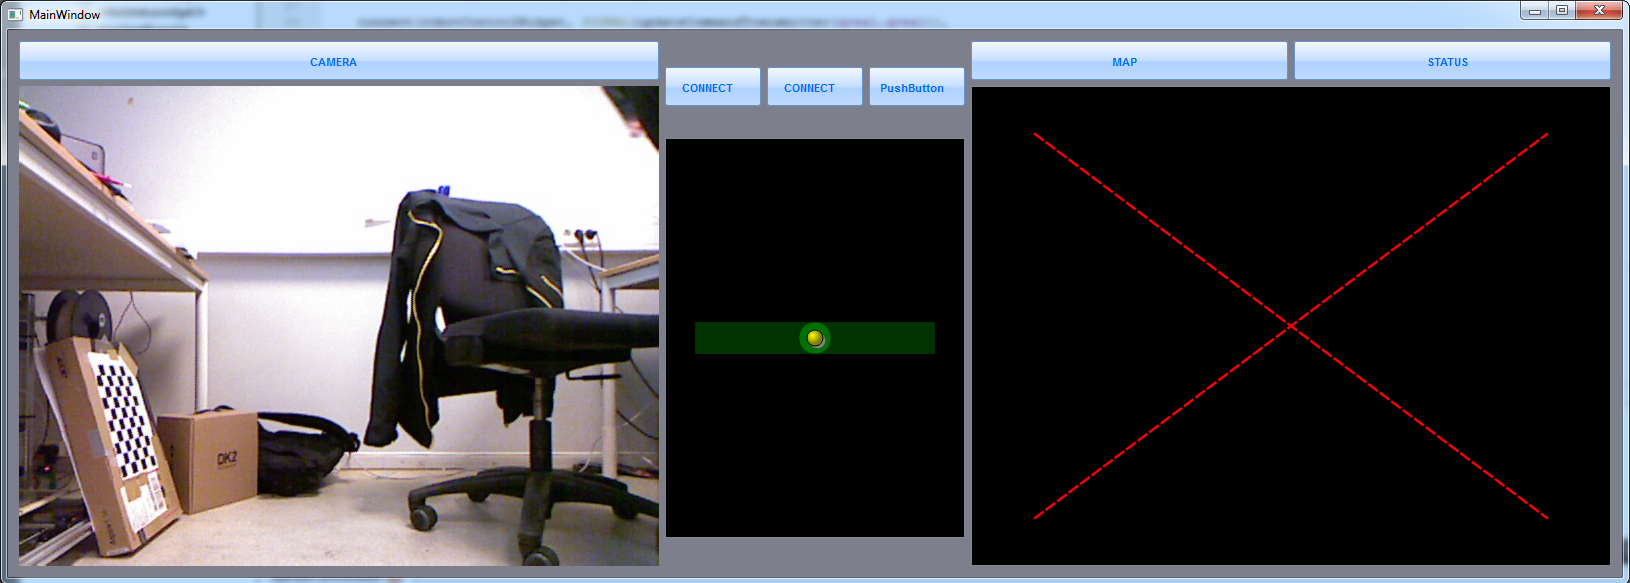
\includegraphics[width=1\textwidth]{basic_ocs_consept}
	\caption{Operator Control Station (OCS) \ac{HMI}. The current skeleton implementation displays live video from the robot. The operator can steer the robot by moving the yellow ball in the center screen. }
	\label{fig:ocs}
\end{figure}


The \ac{OCS} is created with Qt5, a cross-platform framework with a vast set of APIs and a large framework for \ac{GUI} design and development. The \ac{GUI} was planned to consist of three screens: two multi function displays on each side of a control screen. In its current form, only the camera display on the left side is implemented, and the user can interact with a yellow ball on the center screen to control the robot. Code implementation for the center display, \texttt{RobotControlWidget} is based on sample code from the "elasticnodes" example of the Qt Toolkit\footnote{\url{http://doc.qt.io/qt-5/qtwidgets-graphicsview-elasticnodes-example.html}}. The yellow ball is defined by the \texttt{ControlNode} class. The position of the node is subjected to mass-spring-dampener dynamics, to ensure that the ball will return to center when released. Two force vectors $F_x$ and $F_y$ are calculated and applied to the motion equations of the \texttt{controlNode}. Force calculations are performed at a constant rate which defines $\Delta t$ used in the position update calculation.  


\section{The Hand Held Remote Control - \textit{Robot Leash}}

Because the \ac{OCS} is only partially implemented, an operator will not have access to all the features on the robot. In addition, as a safety precaution a person should be close to the robot at all times, and be ready to pull the plug. Furthermore, it is hard to control a moving robot through the on-board keyboard. These problems were countered by the Android-based remote control, \textit{Robot Leash}. This application allows an operator to steer the robot from a mobile device via a Bluetooth connection. Details of the implementation are not included. This section will rather focus on how the mobile application interacts with the robot. A typical use case is as follows (figure \ref{fig:app_screens}):

\begin{enumerate}
	\item The robot is online, and a discoverable Bluetooth server is running on the robot computer.
	\item An operator wishes to control the robot, and starts ''Robot Leash'' on his/her Android device. The operator can now scan for devices within range.
	\item After clicking the \textit{scan} button, the robot is discovered. When the operator selects the discovered device, he/she will be prompted to pair with the robot.
	\item The smartphone and the robot is now paired, and velocity commands from the blue control stick are passed to the robot via Bluetooth. The velocity command switch on the robot, \texttt{velocity\_cmd\_switch}, must be set to \texttt{/cmd\_vel\_bt}.
\end{enumerate}

\begin{figure}[H]
	\centering
	\begin{subfigure}[b]{0.30\textwidth}
		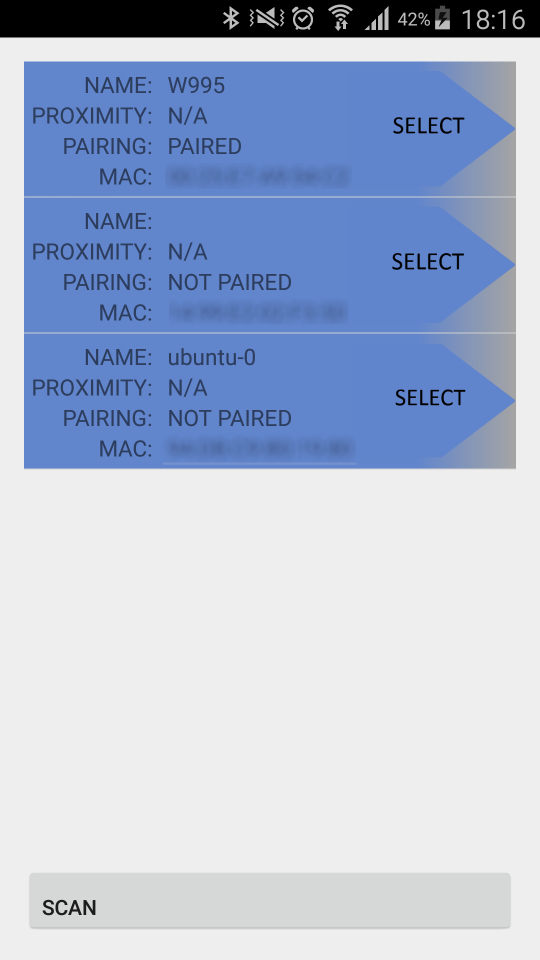
\includegraphics[width=\textwidth]{device_select}
		\caption{First activity with device list.}
		\label{fig:device_select}
	\end{subfigure}
		\begin{subfigure}[b]{0.30\textwidth}
			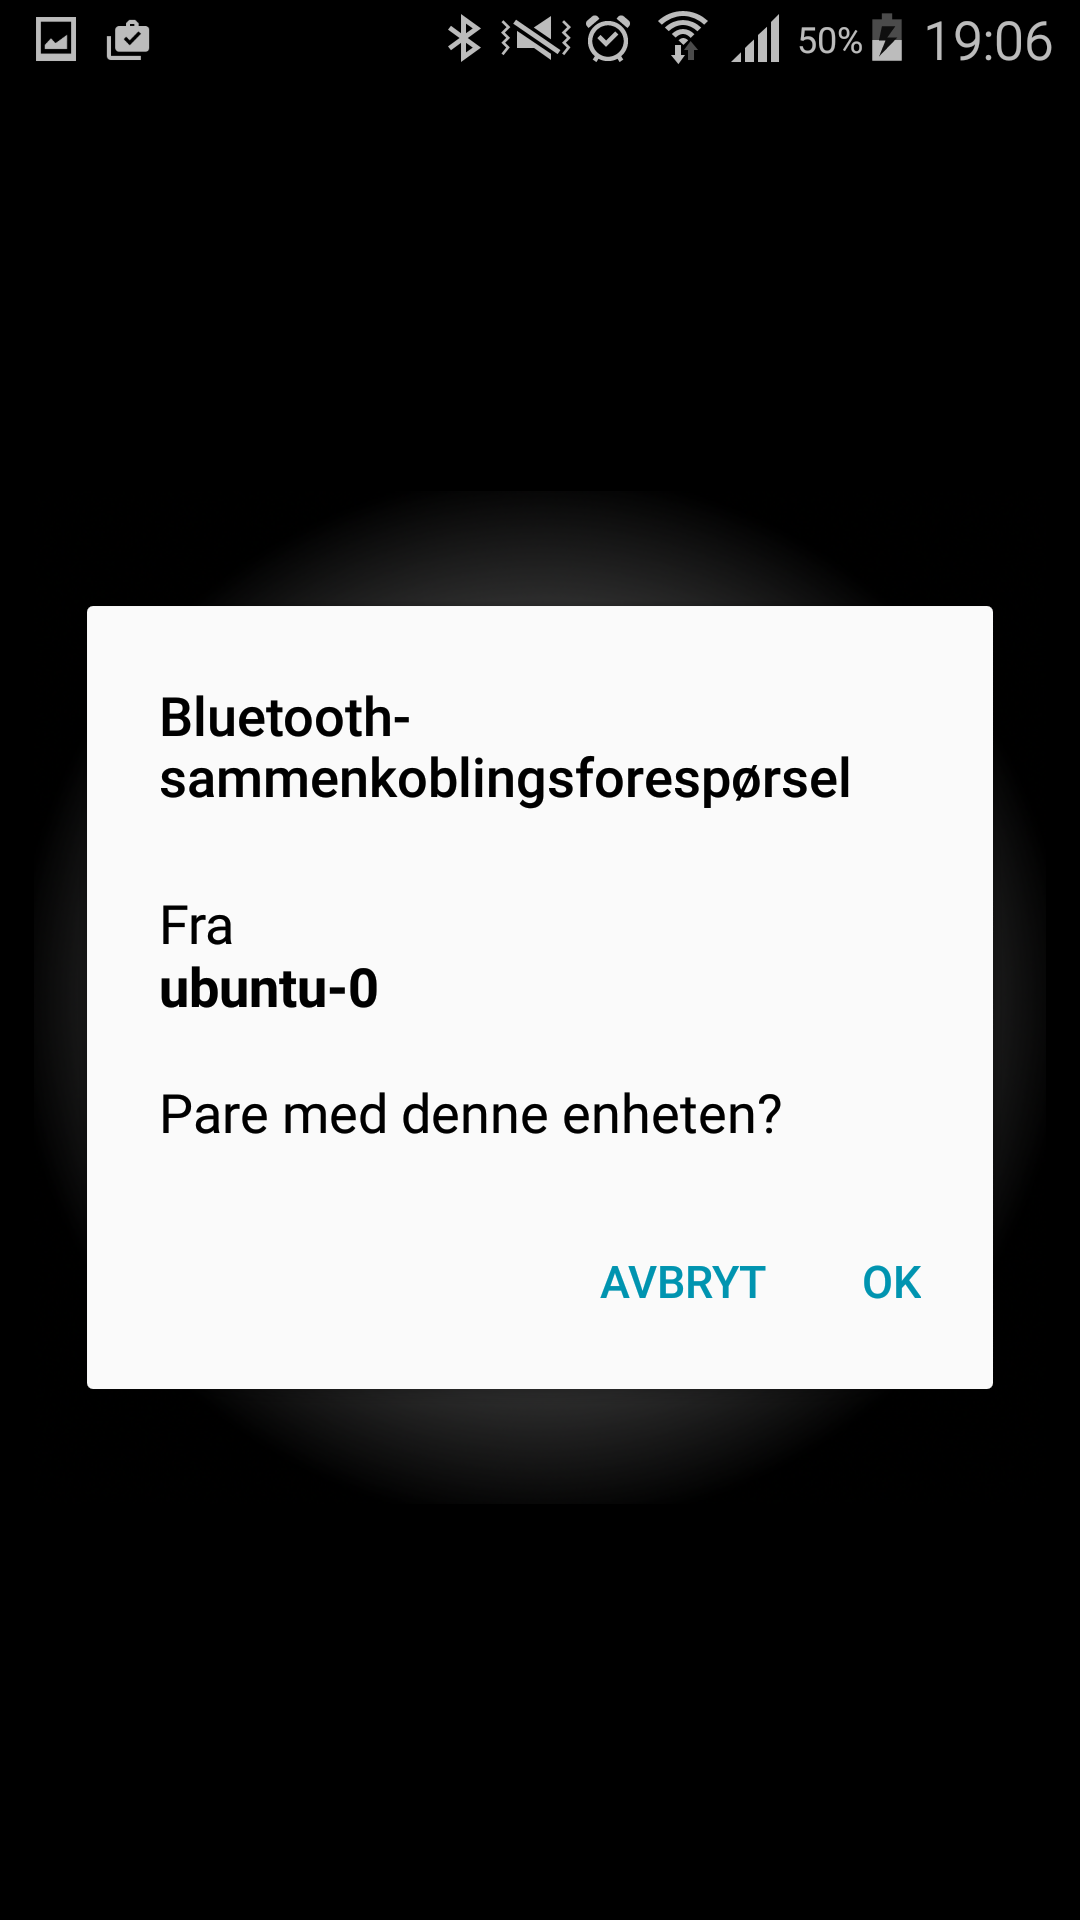
\includegraphics[width=\textwidth]{bt_request}
			\caption{The user is prompted to pair with the robot.}
			\label{fig:bt_request}
		\end{subfigure}
	\begin{subfigure}[b]{0.30\textwidth}
		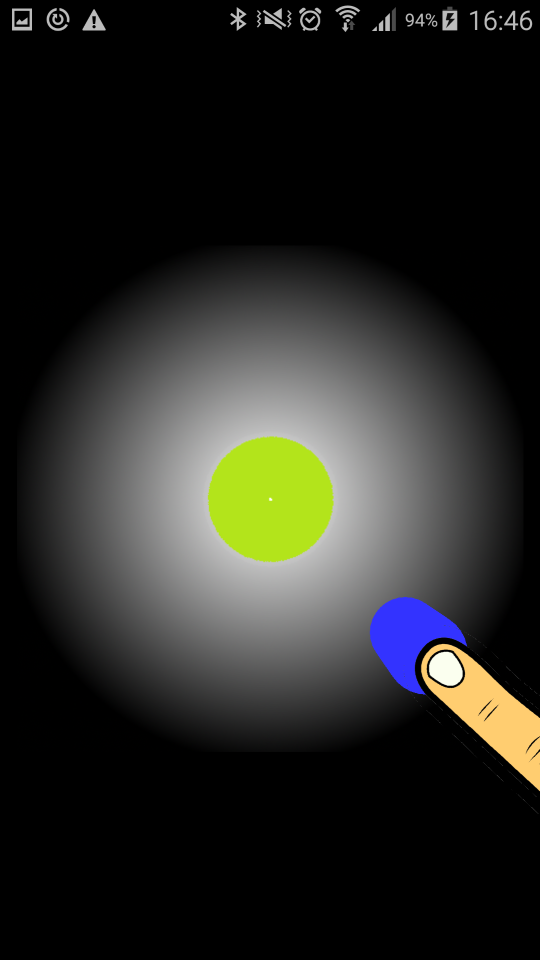
\includegraphics[width=\textwidth]{using_app}
		\caption{Controlling the robot with the stick.}
		\label{fig:using_app}
	\end{subfigure}
	\caption{\label{fig:app_screens}A typical use case for ''Robot Leash''.}
\end{figure}

\subsection{Application Structure}


The \ac{GUI} used to control the robot (figure \ref{fig:using_app}) is implemented in OpenGL ES2. To save time, the code structure behind the graphics is an adaptation from a coding sample in the book \textit{OpenGL ES 2 for Android}\cite{brothaler2013opengl}. The same approach is applied to the portion of the app which manages the Bluetooth connection, i.e. the file \texttt{BluetoothConnectionService.java}. The code within this file is taken from a Bluetooth chat sample\footnote{https://github.com/googlesamples/android-BluetoothChat/...}, provided by Google. 

\subsection{Interaction With the Robot}

Communication between robot and smartphone is done over a Bluetooth connection with a server-client pair. The robot will set up a Bluetooth server, exposing a service with a \ac{UUID}. The Android application can now connect to this specific service. To speed up the implementation process, the service \ac{UUID} has been hard coded into the Android application. It is recommended to implement a more elegant solution later. Figure \ref{fig:android_sequence} shows how a touch gesture by the user is transferred to the robot as velocity commands. 

Android and Qt offers the option to choose either a secure or non-secure connection. The Android reference states that an insecure connection ''not have an authenticated link key''\cite{android_bt_reference}, making it vulnerable to man-in-the-middle attacks. However, for reasons of ease of use, the connections used here are set to non-secure. No further functionality was added besides the ability to send transmit velocity commands. Additional changes were only minor, such as disabling screen rotations when controlling the robot. 

http://developer.samsung.com/technical-doc/view.do?v=T000000117

\begin{sidewaysfigure}[ht]
	\centering
	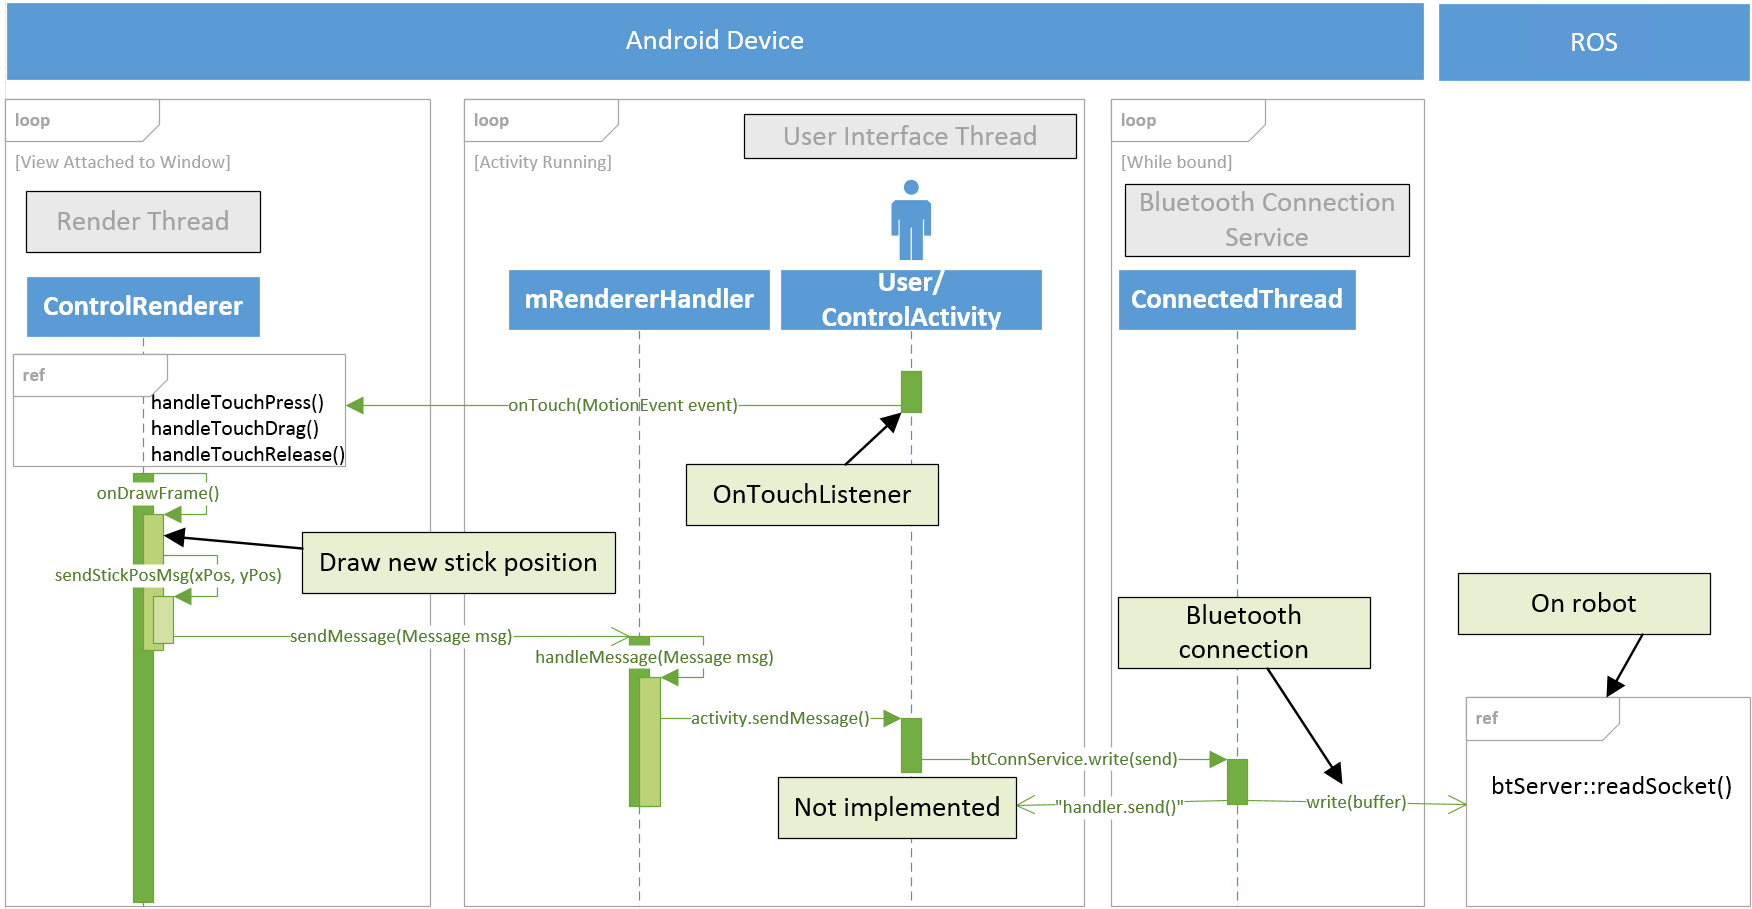
\includegraphics[width=1\textwidth]{android_sequence}
	\caption[This is the caption \newline This is the second line]{\begin{minipage}[t]{.8\linewidth}Sequence diagram illustrating how user touch gestures are detected and propagated \\through the application, before being transmitted as commands to the robot. \end{minipage}}
	\label{fig:android_sequence}
\end{sidewaysfigure}


\section{Mapping - Setting Up RTAB-Map}
\label{sec:mapping}
This robot is using Real-Time Appearence Based Mapping (\ac{RTAB-Map}) for \ac{SLAM}. As mentioned in section \ref{sec:RTAB-Map}, \ac{RTAB-Map} itself has been developed over the last decade by IntRoLab at Université de Sherbrooke in Canada. This section presents how \ac{RTAB-Map} was configured for this robot. In this project, \ac{RTAB-Map} was initially installed in the form of a released binary for \ac{ROS} Indigo. Because of a crippling bug (ref. section \ref{sec:tfException}) which was fixed in the source code
of \texttt{rtabmap\_ros}, but not in the released binary, this package had to be built and installed from source.

\subsection{Configuration}
\label{sec:configuration}
As all \ac{ROS} programs which are a part of the robot system, \ac{RTAB-Map} will run as a node that subscribes and publishes topics. The first task in configuring \ac{RTAB-Map} is to connect the robots sensor data to the \ac{RTAB-Map} node. The node, called \texttt{rtabmap}, can build 2D occupancy grids and/or 3D point cloud representations of the environment. In this project, \ac{RTAB-Map} is configured to do both. The configuration is based on a guide\cite{rtabmap_setup} provided by the developers. To perform \ac{SLAM}, the mapping node subscribes to odometry, 2D laser scans and camera information. There are five possible sensor configurations with the Kinect\cite{rtabmap_setup}:

\subsubsection{1 - Kinect + LIDAR + Odometry} 
Sensor data can be sent directly to \texttt{rtabmap}.

\subsubsection{2 - Kinect + Odometry + Fake 2D laser from Kinect}

2D laser scans are generated by passing depth images from the Kinect through the node \texttt{depthimage\_to\_laserscan}.

\subsubsection{3 - Kinect + LIDAR}

This is the configuration that was used in this project. Odometry data is generated by a the scanmatcher within Hector SLAM (section \ref{sec:hector}). 

\subsubsection{4 - Kinect + Odometry}

This configuration is suitable for uneven surfaces, i.e. when the vehicle is not constrained to a plane. Supports \textit{roll}, \textit{pitch} and \textit{yaw} rotations.

\subsubsection{5 - Kinect}

In this mode, odometry will be generated by the \texttt{rgbd\_odometry} node bundled with the \texttt{rtabmap\_ros} package. This node publishes odometry messages based on feature correspondences in consecutive RGBD images received from the camera.

%\begin{center}
%	\begin{tabular}{ l p{7cm} }
%		\textbf{Kinect + LIDAR + Odometry} & Sensor data can be sent directly to \texttt{rtabmap}.\\
%		\textbf{Kinect + Odometry + Fake 2D laser from Kinect} & 2D laser scans are generated by passing depth images from the Kinect to the node \texttt{depthimage\_to\_laserscan}.\\
%		\textbf{Android Application} & A supporting tool intended to function as a remote control for the robot. The implementation presented here enables the user to control the robot from an Android device via a Bluetooth connection.\\
%		\textbf{Operator Control Station} & A simple Operator Control Station (OCS) based on Qt enables an operator to control the robot via a wireless TCP/IP connection. The \ac{OCS} can display a live video stream from the Kinect sensor. \\
%	\end{tabular}
%\end{center}

\texttt{rtabmap} subscribes to two image topics. One topic for depth images, \texttt{/openni/depth/image\_raw}, and another for the rgb image, \texttt{/openni/rgb/image\_raw}. 

\subsection{Adding 3D Obstruction Detection}

The package \texttt{rtabmap\_ros} contains a 3D obstacle detector in addition to the mapping node \texttt{rtabmap}. To enable 3D obstruction, point cloud data from the Kinect is passed through the nodelet \texttt{obstacles\_detection}. The filtered point cloud is sent to \texttt{move\_base} where it will be used in the local costmap.

\section{Navigation}
\label{sec:navigation}
Autonomous navigation in this project is limited to use of the navigation stack in \ac{ROS}, which was introduced in section \ref{sec:navigation_theory}. The stack will be used in its most basic form. The configuration was initially based on a tutorial at \texttt{ros.org}\footnote{http://wiki.ros.org/navigation/Tutorials/RobotSetup}. The implementation consists of one launch file for the node \texttt{move\_base}, and a set of configuration files for each component within \texttt{move\_base}. Figure \ref{fig:mar_2dnav} shows how these files were structured. As with \ac{RTAB-Map}, the configuration process consist of connecting \texttt{move\_base} to the rest of the network, by deciding which topics it shall subscribe to. 

\begin{figure}[h]
	\centering
	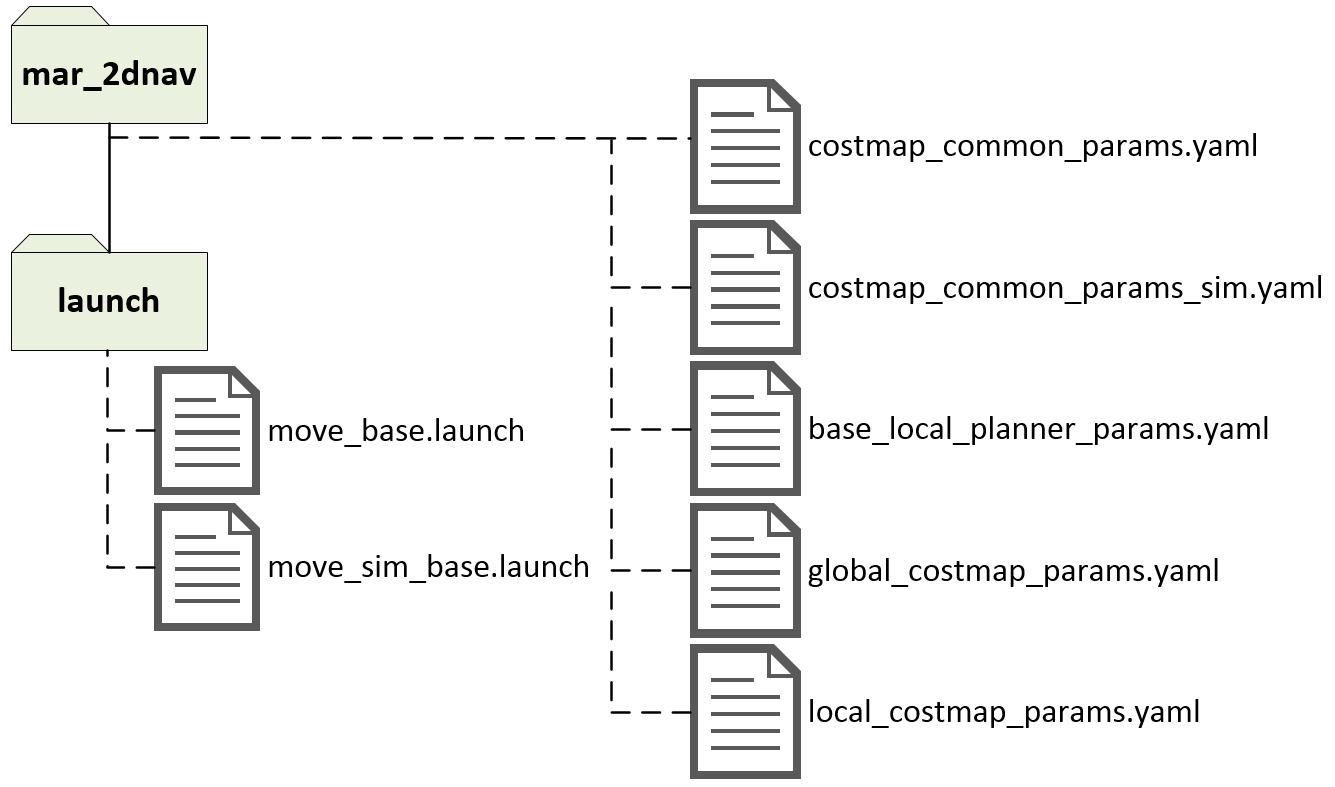
\includegraphics[width=0.8\textwidth]{mar_2dnav}
	\caption{Files for configuring and launching the navigation stack.}
	\label{fig:mar_2dnav}
\end{figure}

\subsection{Local Planner Parameters}

\subsection{Common Costmap Parameters}

As the same costmap package is used for both the local and global costmaps, there are some configuration parameters that are common for these costmaps. The tunable parameters include the robot footprint and the costmap inflation radius. 

\subsubsection{Obstruction Detection}


\begin{figure}
	\centering
	\begin{subfigure}[b]{0.53\textwidth}
		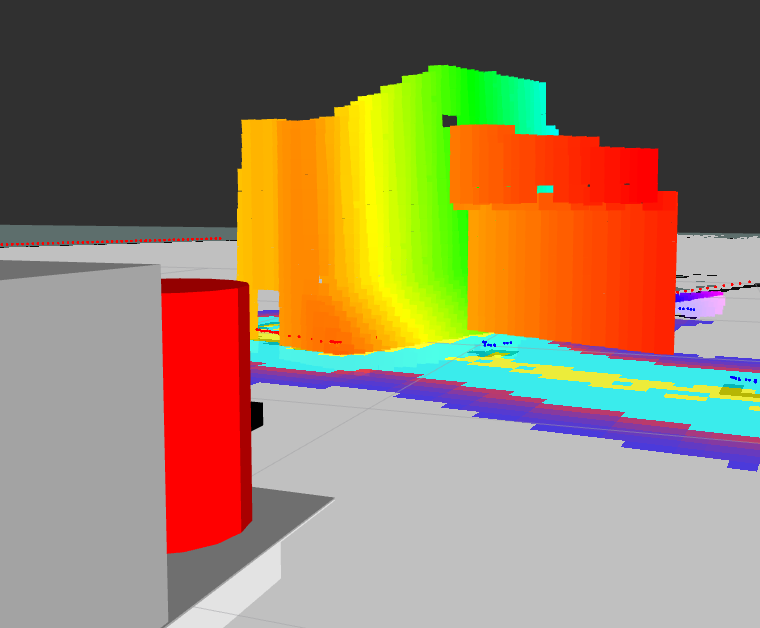
\includegraphics[width=\textwidth]{3d_obstruction1_left}
		\caption{A point cloud representation of the obstruction. Notice how the local costmap is based on the detected point cloud.}
		\label{fig:device_select}
	\end{subfigure}
		\begin{subfigure}[b]{0.45\textwidth}
			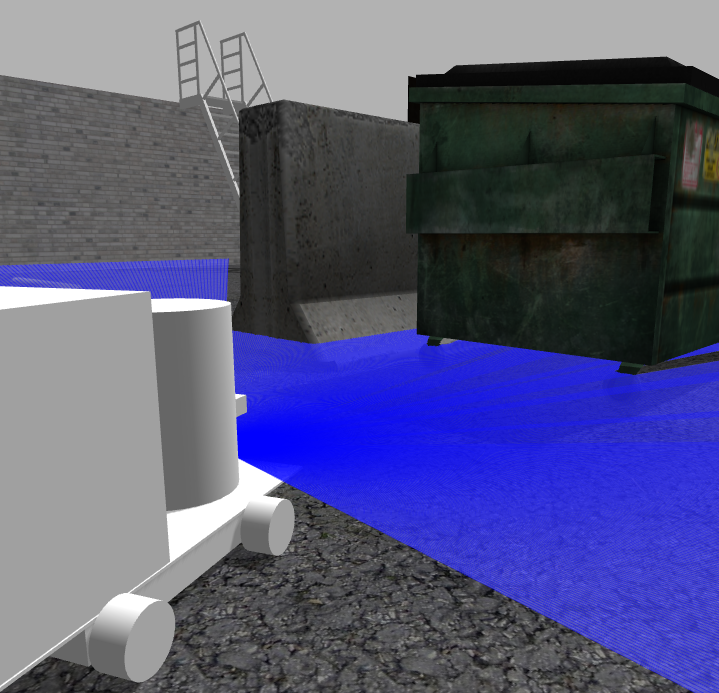
\includegraphics[width=\textwidth]{3d_obstruction1_right}
			\caption{The obstruction in the Gazebo simulator. Notice how the LIDAR only detects the wheels below the container.}
			\label{fig:bt_request}
		\end{subfigure}
	\caption{\label{fig:3d_obstruction1}Detecting obstructions in 3d.}
\end{figure}

\begin{figure}[h]
	\centering
	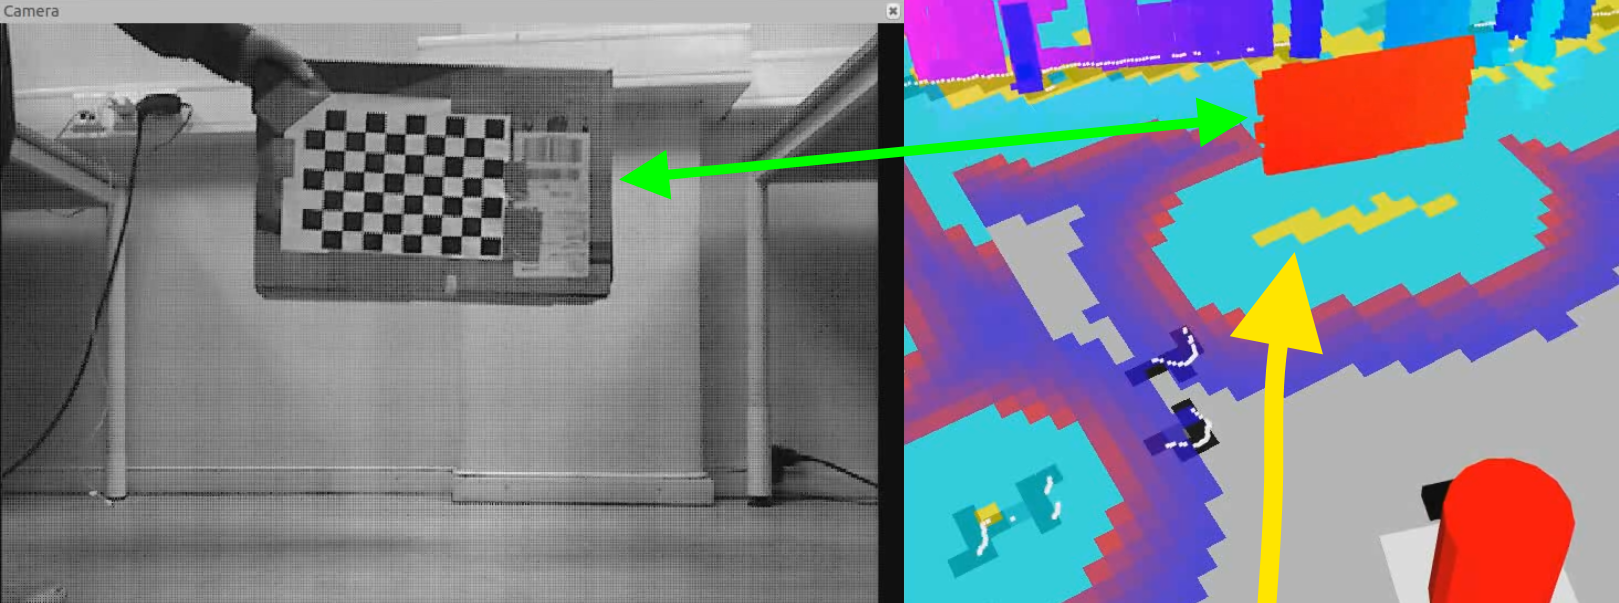
\includegraphics[width=1\textwidth]{live_3d_obstacle2}
	\caption{3D Obstacle detection with the live robot. The nodelet \texttt{obstacles\_detection} filters out the floor and publishes a point cloud which can be sent to the \texttt{move\_base} node. The yellow arrow points to the local cost map, which is based on real-time sensor data and used by the local planner.}
	\label{fig:live_3d_obstacle2}
\end{figure}